%%%%%%%% ICML 2025 EXAMPLE LATEX SUBMISSION FILE %%%%%%%%%%%%%%%%%

\documentclass{article}

% Recommended, but optional, packages for figures and better typesetting:
\usepackage{microtype}
\usepackage{graphicx}
% \usepackage{subfigure}
\usepackage{svg}
\usepackage{pgfplots}
\usetikzlibrary{patterns}
\usepackage{booktabs} % for professional tables
\usepackage{subcaption}
\usepackage{longtable}
\usepackage{tablefootnote}

% hyperref makes hyperlinks in the resulting PDF.
% If your build breaks (sometimes temporarily if a hyperlink spans a page)
% please comment out the following usepackage line and replace
% \usepackage{icml2025} with \usepackage[nohyperref]{icml2025} above.
\usepackage{hyperref}


% Attempt to make hyperref and algorithmic work together better:
\newcommand{\theHalgorithm}{\arabic{algorithm}}

% Use the following line for the initial blind version submitted for review:
% \usepackage{icml2025}

% If accepted, instead use the following line for the camera-ready submission:
\usepackage[accepted]{icml2025}

% For theorems and such
\usepackage{amsmath}
\usepackage{amssymb}
\usepackage{mathtools}
\usepackage{amsthm}

% if you use cleveref..
\usepackage[capitalize,noabbrev]{cleveref}

%%%%%%%%%%%%%%%%%%%%%%%%%%%%%%%%
% THEOREMS
%%%%%%%%%%%%%%%%%%%%%%%%%%%%%%%%
\theoremstyle{plain}
\newtheorem{theorem}{Theorem}[section]
\newtheorem{proposition}[theorem]{Proposition}
\newtheorem{lemma}[theorem]{Lemma}
\newtheorem{corollary}[theorem]{Corollary}
\theoremstyle{definition}
\newtheorem{definition}[theorem]{Definition}
\newtheorem{assumption}[theorem]{Assumption}
\theoremstyle{remark}
\newtheorem{remark}[theorem]{Remark}

% Todonotes is useful during development; simply uncomment the next line
%    and comment out the line below the next line to turn off comments
%\usepackage[disable,textsize=tiny]{todonotes}
\usepackage[textsize=tiny]{todonotes}


% The \icmltitle you define below is probably too long as a header.
% Therefore, a short form for the running title is supplied here:
\icmltitlerunning{Minerva: A Programmable \textit{Memory Test} Benchmark for Language Models}

\begin{document}

\twocolumn[
\icmltitle{Minerva: A Programmable \textit{Memory Test} Benchmark for Language Models}%How capable are LLMs in processing context?}


% It is OKAY to include author information, even for blind
% submissions: the style file will automatically remove it for you
% unless you've provided the [accepted] option to the icml2025
% package.

% List of affiliations: The first argument should be a (short)
% identifier you will use later to specify author affiliations
% Academic affiliations should list Department, University, City, Region, Country
% Industry affiliations should list Company, City, Region, Country

% You can specify symbols, otherwise they are numbered in order.
% Ideally, you should not use this facility. Affiliations will be numbered
% in order of appearance and this is the preferred way.
\icmlsetsymbol{equal}{*}

\begin{icmlauthorlist}
\icmlauthor{Menglin Xia}{equal,ms}
\icmlauthor{Victor R\"{u}hle}{ms}
\icmlauthor{Saravan Rajmohan}{ms}
\icmlauthor{Reza Shokri}{equal,nus}
\end{icmlauthorlist}

\icmlaffiliation{ms}{M365 Research, Microsoft}
\icmlaffiliation{nus}{National University of Singapore}

\icmlcorrespondingauthor{Menglin Xia}{mollyxia@microsoft.com}
\icmlcorrespondingauthor{Reza Shokri}{reza@comp.nus.edu.sg}

% You may provide any keywords that you
% find helpful for describing your paper; these are used to populate
% the "keywords" metadata in the PDF but will not be shown in the document
\icmlkeywords{LLM evaluation, memory test, context utilization, benchmark}

\vskip 0.3in
]

% this must go after the closing bracket ] following \twocolumn[ ...

% This command actually creates the footnote in the first column
% listing the affiliations and the copyright notice.
% The command takes one argument, which is text to display at the start of the footnote.
% The \icmlEqualContribution command is standard text for equal contribution.
% Remove it (just {}) if you do not need this facility.

%\printAffiliationsAndNotice{}  % leave blank if no need to mention equal contribution
\printAffiliationsAndNotice{\icmlEqualContribution} % otherwise use the standard text.

\begin{abstract}
How effectively can LLM-based AI assistants utilize their memory (context) to perform various tasks? Traditional data benchmarks, which are often manually crafted, suffer from several limitations: they are static, susceptible to overfitting, difficult to interpret, and lack actionable insights--failing to pinpoint the specific capabilities a model lacks when it does not pass a test. In this paper, we present a framework for automatically generating a comprehensive set of tests to evaluate models' abilities to use their memory effectively. Our framework extends the range of capability tests beyond the commonly explored (passkey, key-value, needle in the haystack) search, a dominant focus in the literature. Specifically, we evaluate models on atomic tasks such as searching, recalling, editing, matching, comparing information in context memory, and performing basic operations when inputs are structured into distinct blocks, simulating real-world data. Additionally, we design composite tests to investigate the models' ability to maintain state while operating on memory. Our benchmark enables an interpretable, detailed assessment of memory capabilities of LLMs.

%How capable are LLM-based AI assistants in using their context (memory) to perform various tasks? It is known that Data benchmarks, which are mostly manually crafted, are static, prone to being overfitted on, not so interpretable and not actionable (they do not suggest what exact capabilities are missing if the model fail the tests). In this paper, we design a framework to automatically generate a range of atomic and composite tests to gauge the capabilities of the models in using their context. Our framework significantly expands the set of capabilities beyond simple key-value search capability which is used in the literature. We evaluate models' ability to search, recall, edit, match, compare information in the context memory, and perform simple operations when the input is structured into different blocks (which represent how in real world data is created). We also test how the models can keep state as parsing the context memory. 
\end{abstract}


\section{Introduction}
\label{sec:intro}
% Image editing methods in diffusion models depend on user-defined control directions - users can unlock their creativity using these methods by specifying the desired manipulation through prompts~\cite{gandikota2023concept}, reference images~\cite{ruiz2022dreambooth, kumari2022customdiffusion, gal2022image, chen2024trainingfreeregionalpromptingdiffusion}, or attribute vectors~\cite{parmar2023zero,hertz2022prompt}. In this work, we ask a fundamentally different question: \emph{Can we automatically discover the underlying visual structure of a concept within diffusion model's knowledge?} %Rather than requiring user-specified controls, we aim to decompose the model's internal knowledge into meaningful directions.

% This question touches on a fundamental limitation in how we interact with diffusion models. Current control methods ~\cite{zhang2023addingconditionalcontroltexttoimage, gandikota2023concept, ye2023ipadaptertextcompatibleimage,ye2023ipadaptertextcompatibleimage, hertz2024stylealignedimagegeneration, li2023photomaker, shi2024instantbooth, chen2024trainingfreeregionalpromptingdiffusion} require users to specify their desired manipulations in advance, limiting interactive creativity. This contrasts with natural human artistic workflows, where creators dynamically explore creative ideas while jointly refining them toward meaningful artistic outcomes~\cite{hoffmann2016modeling}. This synergy between specification and exploration is not new to generative models. Early GAN architectures naturally developed disentangled latent spaces that enabled continuous\cite{harkonen2020ganspace,radford2015unsupervised, wu2021stylespace, shen2020interfacegan}, compositional control over generated images. Users could explore these spaces to discover interesting variations that would be difficult to describe in words~\cite{wu2021stylespace}, then combine them to achieve their creative goals~\cite{grabe2022towards}. 


% While diffusion models have largely superseded GANs in conditional image synthesis~\cite{dhariwal2021diffusion},  their underlying structure remains less understood. Diffusion models achieve remarkable diversity through high-dimensional latents, unlike GANs' compact latent spaces.  With a single prompt, diffusion models can generate radically different variations through different random initializations of input noise. We ask - Is it possible to discover interpretable structure within this vast space of variations?

Text-to-image diffusion models are capable of generating remarkable visual variations from a single prompt through different random initializations. However, this vast creative potential remains largely opaque to users---while we can generate diverse images, we lack understanding of the underlying structure of these variations. This presents a fundamental challenge: how can we discover and expose the latent visual capabilities encoded within these models?

\let\thefootnote\relax \footnote{$^{*}$Correspondence to \texttt{gandikota.ro@northeastern.edu}}

The challenge touches on a key limitation in how we interact with diffusion models today. Current control methods require users to explicitly specify their desired edits in advance through prompts~\cite{gandikota2023concept}, reference images~\cite{zhang2023addingconditionalcontroltexttoimage, chen2024trainingfreeregionalpromptingdiffusion, ruiz2022dreambooth,kumari2022customdiffusion, Ryu_lora, hu2021lora}, or attribute vectors~\cite{ye2023ipadaptertextcompatibleimage, hertz2024stylealignedimagegeneration, li2023photomaker, shi2024instantbooth,parmar2023zero,hertz2022prompt}. That contrasts sharply with natural human creative workflows, where artists dynamically explore creative ideas and jointly refine them toward meaningful artistic outcomes~\cite{hoffmann2016modeling}. The need for pre-specified controls creates a barrier between users and the full creative potential of these models.

Interestingly, earlier generative models like GANs~\cite{gans,karras2019style,brock2018large} naturally developed more interpretable internal structures. Their compact latent spaces often exhibited emergent disentanglement~\cite{harkonen2020ganspace,radford2015unsupervised, wu2021stylespace, shen2020interfacegan}, enabling continuous and compositional control over generated images. Users could explore these spaces to discover interesting variations that would be difficult to describe in words~\cite{wu2021stylespace}, then combine them to achieve their creative goals~\cite{grabe2022towards}.

Diffusion models have largely superseded GANs in conditional image synthesis~\cite{dhariwal2021diffusion}, achieving greater diversity through much higher-dimensional latents. And yet an understanding of the underlying structure of these larger latent spaces has remained elusive. In this work, we ask a fundamental question: \emph{Can we automatically discover the visual structure within a diffusion model's knowledge of a concept?} Rather than requiring user-specified controls, we aim to decompose the model's internal representations into expressive directions that users can explore and combine.

To address these needs, we present \textbf{SliderSpace}, a framework that brings systematic explorability to diffusion models. Given just a text prompt, SliderSpace discovers a canonical set of meaningful, diverse, and controllable directions within the model's knowledge of that concept. Each direction is implemented as a low-rank adapter~\cite{hu2021lora} that can be scaled and composed with others, allowing users to explore and smoothly combine different aspects of variation, as shown in Figure~\ref{fig:intro}.

We ground SliderSpace discovery in three key requirements for meaningful decomposition of a diffusion model's visual manifold: 
\begin{enumerate}
    \item \textbf{Unsupervised Discovery:} The decomposition process should emerge from the intrinsic structure of the model's learned representation, rather than being guided by predefined attributes. This ensures we capture the true topology of the model's knowledge space rather than projecting our assumptions onto it.
    
    \item \textbf{Semantic Orthogonality:} Each discovered control must represent a distinct semantic direction. This is enforced in a semantic feature space, like CLIP, where every slider has an orthogonal effect in embeddings. This prevents discovering multiple controls that create similar semantic effects, making the system more efficient and easier.
    
    \item \textbf{Distribution Consistency:} Directions must induce consistent transformations across both random seeds and prompt variations. 
\end{enumerate}

These requirements naturally lead to our proposed framework, which we formalize in Section~\ref{sec:method}. As we show in our experiments, SliderSpace is architecture-agnostic, working with both conventional U-Net based models like Stable Diffusion~\cite{rombach2022high, rombach2022sd20, podell2023sdxl, turbo, dmd} and recent transformer-based architectures like Flux~\cite{flux}.

We demonstrate the expressiveness of SliderSpace through three applications: First, we show how SliderSpace can decompose high-level concepts into diverse and expressive components, revealing the natural axes of variation in the model's understanding. Second, we explore artistic style variation, where SliderSpace discovers directions that match or exceed the diversity of manually curated artist lists while being judged more useful by human evaluators. Finally, we show how SliderSpace can help reverse the mode collapse commonly observed in distilled diffusion models, restoring diversity while maintaining generation speed.

Beyond providing practical creative control, SliderSpace opens new avenues for understanding and utilizing the latent capabilities of diffusion models. By mapping these models' visual potential into intuitive, composable directions, we take a step toward making their creative possibilities more accessible and interpretable to users.

% Image editing methods in diffusion models unlock the creativity of users. In this work we ask an alternate question: \emph{Can we organize and expose what of the diffusion model is already capable of?}.
% Existing methods for controlling image generation typically require users to manually specify edit directions for desired changes. This process is time-consuming, requires technical expertise, and limits the spontaneity of the creative process. For instance, if a user wants to adjust the smile of a generated person, they must explicitly request this edit, often through imprecise prompt engineering or model fine-tuning. This approach of predefined controls or manual specifications restricts users from fully exploring the latent capabilities of the model. There may be interesting stylistic variations or attributes that the model can generate, but users have no easy way to discover or utilize these.

% Natural visual disentanglement was an emergent property in the latent space of Generative Adversarial Models (GANs) \cite{harkonen2020ganspace,radford2015unsupervised, wu2021stylespace, shen2020interfacegan}. In particular, it has been observed that StyleGAN~\cite{karras2019style} stylespace neurons offer detailed control over many meaningful aspects of images that would be difficult to describe in words~\cite{wu2021stylespace}. However, diffusion models do not share such a compact latent space~\cite{park2023unsupervised}; and efforts to uncover such a space in the semantic embeddings of the text conditioning have met with limited success \nik{Nick - is there a specific citation you were thinking about?}.

% In this work we introduce \textbf{SliderSpace}, which takes a step towards uncovering an analogous low dimensional representation of diffusion models' visual breadth; in essence treating the diffusion model as many generators sharing parameters, where a particular generator is defined by a specific prompt. For a given prompt we sample many random seeds (and optionally prompt expansions using an LLM), generate the corresponding images, and apply an off the shelf feature extractor (in this work CLIP, but our method can be applied to any differentiable feature extractor). We use PCA to analyze these features, and for each of the leading $k$ principal components we train a LoRA \cite{} which causes the diffusion model to produces images which increase the feature magnitude along that component when passed back through the same feature extractor. This leads to a 'Slider' for each principal component, because each LoRA can be scaled and applied to the original diffusion model, continuously varying those visual features in the generated results (as measured, in our case, by CLIP).

% There are many other works that enhance the controllability of diffusion models. One common approach is enabling users to add spatial constraints to a generation either manually, or via a reference image \cite{zhang2023addingconditionalcontroltexttoimage, chen2024trainingfreeregionalpromptingdiffusion}, a second is leveraging more abstract embeddings (e.g. identity, style) extracted from a reference image \cite{ye2023ipadaptertextcompatibleimage, hertz2024stylealignedimagegeneration, li2023photomaker, shi2024instantbooth}, a third is finetuning a foundation model to better generate a concept important to the user \cite{ruiz2022dreambooth, kumari2022customdiffusion, Ryu_lora, hu2021lora}, and a fourth (most relevant to this work) is finding low-rank adaptors of the model based on a prompt or small training set which can be scaled to provide continous control over one aspect of generated image (e.g. night vs day, basic vs luxury, etc.) \cite{gandikota2023concept}. SliderSpace is complementary to all of these methods and offers something distinct. All of the other methods we are aware require the user (and / or model designer) to know in advance what type of control they want. In contrast SliderSpace assists users in discovering and controlling hidden capabilities present in the diffusion model's distribution of possible generations.

%We propose that truly intuitive creative control in a text-to-image model should meet three key criteria: \emph{discoverability}, \emph{intuitiveness}, and \emph{specificity}. The model should reveal controllable attributes that may not be immediately obvious, offer controls that are easy to understand and manipulate, and ensure each control affects a distinct attribute of the generated image.

% We demonstrate the utility and power of SliderSpace using three applications built on top of SDXL-DMD \cite{dmd}, because its fast generation speed lends itself well to the continuous control offered by SliderSpace.

% First, we study concept decomposition (Section \ref{sec:concept_exp}), where we learn sliders for a specific concept (e.g. 'monster', 'waterfall', 'car'). Through quantitative metrics of diversity and text alignment we demonstrate that the learned sliders dramatically boost the diversity of generations when randomly applied without harming text alignment; we also ask humans to qualitatively judge these results in a user study where they find the SliderSpace results to be more 'Diverse', 'Useful', and 'Creative' than our baselines.

% Second, we attempt to compare the automatic discoveries of SliderSpace to a large scale manual study of artistic styles (Section \ref{sec:art_exp}), open-sourced by ParrotZone \cite{parrotzone}. In this study SDXL was prompted with over 4300 artist names,  and based on visual inspection the cases of successful stylistic mimicry recorded. Quantitatively SliderSpace more closely matches the distribution of artistic variation discovered by ParrotZone than other baselines, and in our user studies was judged to be significantly more 'Diverse' and 'Useful' than the baselines. To our surprise humans even judged SliderSpace results to be slightly more 'Diverse' than the results generated by the manually discovered artist names of \cite{parrotzone}.

% Third, we attempt to use SliderSpace to reverse the mode collapse commonly observed in distilled few-step diffusion models relative to the original teacher model (Section \ref{sec:diverse_exp}). We quantitatively demonstrate that applying SliderSpace to SDXL-DMD leads to more closely matching the distribution of images by the original teacher, SDXL.

%Through extensive experiments on various state-of-the-art text-to-image models, we demonstrate that SliderSpace significantly enhances user control and creative expression in AI-assisted image generation tasks. Our method enables a range of applications, including concept decomposition and control, diversity improvement in generated images, customization dissection and edits, and the exploration of artistic styles inherent in the model.

% SliderSpace goes beyond providing a practical tool for enhanced creative control. By mapping the visual potential of diffusion models it can open new avenues for generative creativity and deepens our understanding of each model's hidden potential.
\section{Physical Coherence Benchmark}



\subsection{Prompts}
To comprehensively evaluate the physical coherence of text-to-video generation models, we propose a benchmark set containing 120 prompts, categorized into seven groups: (1) gravity, (2) collision, (3) vibration, (4) friction, (5) fluid dynamics, (6) projectile motion, and (7) rotation. Some examples are shown in Table \ref{tab:example_prompts}. We reference definitions and explanations of motion from physics textbooks from a professional standpoint, while also considering common motion scenarios in action recognition datasets such as UCF101\cite{ucf101}, PennAction\cite{pennaction}, and HAA500\cite{haa500} from an everyday perspective. Ultimately, based on these references, we classify motions into seven categories. Our prompts can also be grouped into three types based on their content: (1) simulated physical experiments (e.g., "A rubber duck falls freely from a height and lands on the wooden floor."), (2) common physical phenomena in daily life (e.g., "A swing is pulled to the highest point and then released, beginning to sway."), and (3) object movements in sports activities (e.g., "A ping pong ball falls from a height onto a table and bounces."). The statistics for these prompts, in terms of their distribution across the seven categories, are shown in Figure~\ref{fig:prompt}.








\subsection{Human Evaluation Results}
We evaluated four text-to-video generation models (Keling1.5 \cite{keling}, Gen-3 Alpha \cite{runway}, Dream Machine \cite{luma}, and OpenSora-STDiT-v3 \cite{opensora}) by generating videos based on our 120 prompts. Some of the generated video results are shown in Figure~\ref{fig:sota_vis}. It is evident that the generated videos do not consistently adhere to physical consistency. For the same prompt, the quality of the videos varies significantly across the four models. This indicates that there is still a substantial gap between different models in terms of physical consistency. Therefore, there is an increased need for a more accurate and in-depth evaluation of model performance in this dimension.



\begin{figure}[ht]
\centering
\includegraphics[width=0.8\linewidth]{figures/rank_all.pdf}
\caption{\textbf{Overall ranking result from manual evaluation.}}
\label{fig:rank_all}
\end{figure}

\begin{figure}[ht]
\centering
\includegraphics[width=0.8\linewidth]{figures/rank_c.pdf}
\caption{\textbf{Category-specific ranking results from manual evaluation.}}
\label{fig:rank_c}
\end{figure}


For the videos generated by the four T2V models, we initially conduct a manual ranking of the four models for each prompt. The results are shown in Figure~\ref{fig:rank_all} and Figure~\ref{fig:rank_c}. 

In Figure~\ref{fig:rank_all}, the physical coherence performance of the four T2V models was manually evaluated and ranked. As shown in the figure, Keling1.5 stands out with the highest physical coherence, significantly outperforming the other models. The performances of Dream Machine and Gen-3 Alpha are quite close to each other. In contrast, the open-source model OpenSora-STDiT-v3 scores relatively lower, far behind the top three, indicating substantial room for improvement in terms of physical coherence.

Figure~\ref{fig:rank_c} presents the detailed performance of each model across the seven physical scenario categories. In this radar chart, Keling1.5 demonstrates the most comprehensive performance, covering the widest range, and achieves the highest scores in several categories, particularly excelling in gravity, collision, and friction. Dream Machine and Gen-3 Alpha show relatively balanced performance but are slightly behind. OpenSora-STDiT-v3, on the other hand, performs relatively poorly, failing to achieve high scores across all categories.

The drawback of manual evaluation is the lack of quantifiable metrics for comparison, as well as the high cost. Therefore, we use a frame prediction model for automated quantitative evaluation. Next, we will provide a detailed introduction to the frame prediction model.

\begin{figure*}[t]
  \centering
  \vspace{-1pt}
   \includegraphics[width=0.99\linewidth]{figures/infer_pipe.pdf}
   \vspace{-5pt}
   \caption{
   \textbf{Inference process of PhyCoPredictor.} Once we obtain the generated video from the T2V model, we input the first frame and the prompt into PhyCoPredictor. The Latent Flow Diffusion Module predicts the future optical flow, which then guides the Latent Video Diffusion Module to predict future video frames.}
   \label{fig:infer_pipe}
   \vspace{-1pt}
\end{figure*}
\section{Evaluation}
% \begin{figure*}[t!]
    \centering
    \begin{subfigure}[t]{0.45\textwidth}
        \includegraphics[width=0.9\textwidth]{images/black_box_radar.png}
        \caption{Performance of the black-box models.}
        \label{fig:first}
    \end{subfigure}
    \begin{subfigure}[t]{0.45\textwidth}
        \includegraphics[width=0.9\textwidth]{images/white_box_radar.png}
        \caption{Performance of the open-source models.}
        \label{fig:second}
    \end{subfigure}
    \caption{Overall performance of nine models on a snapshot within 4k context length of Minerva.}
    \label{fig:radar}

\end{figure*}

\subsection{Experimental Setup}
We use the proposed framework to evaluate nine widely used language models on a fixed snapshot of 1110 randomly generated test samples. For all tests, we fixed the context length to 4k tokens, except in the Stateful Processing category, where the context length depends on the number of operation steps. We set the number of steps as 200 for quantity state and 100 for set state, corresponding to an approximate context length of 1.5k tokens. For evaluation, we use exact match accuracy for binary tasks, ROUGE-L\citep{lin-2004-rouge} for tests that require sequence overlap measurement, and Jaccard similarity \citep{jaccard1901etude} for set overlap. Further details on the number of examples, hyperparameter configurations, and evaluation metrics for the tests are provided in Appendices \ref{apd:task_detail} and \ref{apd:eval}.

The evaluated models are divided into two groups: 

\textbf{Black-box models}: GPT-4-turbo, GPT-4o, GPT-4o-mini, and Cohere-command-rplus. 

\textbf{Open-source models}: Mistral-7b-instruct-v02, Phi-3-small-128k-instruct (7B), LLaMA-3.1-8b-instruct, Gemma-2-9b, and Phi-3-medium-128k-instruct (14B).

We set the max output token to 4096, temperature to 0, and top\_p to 1 for all model inference.



\subsection{Model Performance Overview}

Figure \ref {fig:radar} summarizes the overall performance of the evaluated models on the memory test snapshot within 4k context length. Notably, this context length is usually considered short for context utilization benchmarks, and many models are expected to perform perfectly at this length. However, our evaluation reveals significant disparities in performance across the capabilities, even within this manageable context length. Overall, the GPT-4-turbo/GPT-4o models show stronger all-around performance across the capabilities. In contrast, other models excel at the search task but struggle significantly in other areas, leading to a widening performance gap compared to stronger models. This is especially evident in the \textbf{Stateful Processing} tasks, where models exhibit steep performance drops. Even within the GPT-4(o) models, there were noticeable variations in performance across different tasks, despite them being the best-performing models. This suggests that strong performance in simple retrieval tasks does not imply effective context processing, highlighting that using NIAH-like tests alone for evaluating context utilization is not sufficient to capture the full spectrum of model capabilities. Our framework instead reveals significant variability in performance across distinct capability categories, offering a more nuanced understanding of model limitations.

The following sections analyze each test type in detail, highlighting key insights from the evaluations.


\subsection{Analysis on Atomic Tests}


\section{Structure Search with Program Synthesis}\label{sec:algo}
%
\subsection{Preliminaries}
\begin{definition}[Tensor, Tensor Size]
Let $d \in \nat$ and $n_1, n_2, \ldots, n_d \in \nat$.
%
A tensor $\ten{T} \in \real^{n_1 \times n_2 \times \cdots \times n_d}$ is a $d$-dimensional array.
%
Each dimension $\mu \in \{1, 2, \ldots, d\}$ has a name $I_\mu$ and $\size{I_\mu} = n_\mu$.
%
We use $\ten{T}_{i_1, i_2, \ldots, i_d}$ to denote an element in the tensor where $i_\mu \in \{1, \ldots, n_\mu\}$.
%
The size of the tensor $\ten{T}$ is defined as $\size{\ten{T}} = \prod_{\mu=1}^{d} n_\mu$.
\end{definition}

\begin{definition}[Matricization]
For a $d$-dimensional tensor $\ten{T} \in \real^{n_1 \times n_2 \times \cdots \times n_d}$ and a set of dimensions $\ind_s \subseteq \{I_1,\ldots, I_d\}$, let $\ind_t = \{I_1, \ldots, I_d\}\ \backslash\ \ind_s$ be the complementary mode set, $\ten{T}' = \mathtt{permute}\left(\ten{T}, [\mu]_{I_\mu \in \ind_s} + [\nu]_{I_\nu \in \ind_t}\right)$ be the permuted tensor with the modes $s$ at the front, then the corresponding \emph{$\ind_s$-matricization} $\matric{T}{\ind_s}$ is defined as $
\matric{T}{\ind_s} = \mathtt{reshape}\left(\ten{T}', \prod_{I_\mu \in \ind_s} n_{\mu}, \prod_{I_\nu \in \ind_t} n_{\nu}\right)$.
\end{definition}
\begin{definition}[Tensor Network]
A tensor network is an undirected graph $G=(\nodes,\edges)$ where each vertex in $\nodes$ is a tensor and each edge in $\edges$ is a tuple of three elements: two node names and their shared index name. Particularly, tensor networks without cycles are called \emph{tree tensor networks}. The tensor represented by a graph $G$ is the contraction of all tensors over shared modes, denoted by $\net{G}$. The size of a tensor network is $\size{G} = \sum_{\ten{T} \in \nodes} \size{\ten{T}}$.
\end{definition}
%
Given a tensor network $G$, we call edges with a dangling end \emph{free edges}, and those without dangling ends \emph{contracted edges}.
%
For example, the network in \autoref{fig:example-program} has four free edges $I_1, I_2, I_3, I_4$ and three contracted edges $r_1, r_2, r_3$.
%
The tensor represented by this network is computed as
$
\net{G}_{ijkl} = \sum_{a=1}^{r_1}\sum_{b=1}^{r_2}\sum_{c=1}^{r_3} \ten{A}_{ia}\ten{B}_{jb}\ten{C}_{abc}\ten{D}_{c k l}
$

\begin{definition}[Tensor Network Structure Search]
The tensor network structure search (TN-SS) problem finds the optimal tensor network that reduces the storage space while maintaining accuracy. Specifically, given a TN-SS problem $(\ten{T}, \error)$ where $\ten{T}$ is the data tensor and $\error$ is a prescribed error bound, the goal of the TN-SS algorithm is to solve the following optimization problem
$$
\arg\min_{G} \quad \size{G} \quad
\textrm{s.t.} \quad \norm{\net{G} - \ten{T}}\leq \error\norm{\ten{T}}
$$
\end{definition}
In other words, the TN-SS problem aims at finding the most compressed tensor network within a given error bound.
%
In this work, we target arbitrary tree structures and do not consider structures with cycles.

\begin{algorithm}[t]
\small
\captionsetup{font=small} % set size of caption font
\caption{Tensor network structure search algorithm}\label{alg:high-level}
\begin{algorithmic}[1]
    \Require The data tensor $\ten{T}$, the error bound $\error$, the param $k$
    \Ensure The result tensor network $G$ such that $\size{G} \leq \size{\ten{T}}$, and $\norm{\net{G} - \ten{T}} \leq \error \norm{\ten{T}}$
    \Function{SearchStructure}{$\ten{T}, \error, k$}
        \State $G_0 \gets (\{\ten{T}\}, \emptyset)$
        \State $G_{min} \gets G_0$
        \For{$(G, \error') \in \textsc{Synth}(\ten{T}, \error, k)$}
            \State $G \gets$ \Call{Round}{$G, \error'$}
            \If{$\size{G} < \size{G_{min}}$}
                \State $G_{min} \gets G$
            \EndIf
        \EndFor
        \State \Return $G_{min}$
    \EndFunction
\end{algorithmic}
\end{algorithm}

\subsection{From TN-SS To Program Synthesis}\label{sec:algo:program}
%
To solve a TN-SS problem $(\ten{T},\error)$, we propose to find a near-optimal solution by generating a transformation program that incrementally splits nodes to produce a tensor network with reduced size.
%
The algorithm that integrates program synthesis with TN-SS is presented in~\cref{alg:high-level}.
%
The process begins by constructing an initial graph $G_0$ containing a single node $\ten{T}$.
%
Then, the algorithm enters a loop, where it repeatedly calls the function \textsc{Synth} (Line 4).
%
This function uses a program synthesizer to enumerate and execute transformation programs, generating various tensor networks $G$.
%
At the end of each iteration, the algorithm calls the procedure \textsc{Round} for further compression, and updates the current minimum structure $G_{min}$ if the newly generated structure has a lower cost.
%
Finally, the algorithm returns the structure with the minimum cost.
%
In the remaining section, we introduce the design of the transformation language and the formal reduction of TN-SS to program synthesis.

\begin{figure}[t]
    \centering
    \small
    \vspace{-1em}
    \begin{alignat*}{2}
        \text{Programs or sketches}\quad & P,\sketch && := \emptyprog \mid \expr \mid \seq{P}{\expr} \\
        \text{Expressions}\quad & \expr &&:= \osplit(\ind, r) \\
        \text{Index sets}\quad & \ind  &&:= \{I_\mu\} \mid \ind \cup \{I_\mu\} \\
        \text{Ranks or holes}\quad & r     &&:=\ \hole \mid 1 \mid 2 \mid \cdots \\
        \text{Dimensions}\quad & \mu   &&:= 1, 2, 3, \ldots
    \end{alignat*}
    \vspace{-2em}
    \begin{align*}
    \sem{E}(\bot) = \bot \quad&\quad \sem{\emptyprog}(G, \error) = (G, \error) \\
    \sem{\osplit(\indices, r)}(G, \error) &= \textsc{ExecOSplit}(G, \error, \ind, r)\\
    \sem{\seq{P}{\expr}}(G,\error) &= \sem{\expr}(\sem{P}(G,\error))
    \end{align*}
    \vspace{-2em}
    \caption{Syntax and semantics for the DSL.}\label{fig:dsl}
    % \vspace{-1em}
\end{figure}

\paragraph{Syntax and Semantics of the Language}
%
As illustrated in~\cref{fig:dsl}, a program $P$ can either be empty, denoted by $\emptyprog$, or a sequence of expressions $\seq{P}{E}$.
%
Each expression represents a split operation that takes a set of indices $\ind$ and a rank $r$ as inputs.
%
The index set consists of indices from different modes $I_\mu$.
%
The rank $r$ can be either an integer or a hole $\hole$, which can be filled later.
%
If a program consists of ranks as holes, it is referred to as a \emph{program sketch}.
%
A sketch $\sketch$ can be completed with a rank assignment $\many{\hole_s \mapsto r_s}$ (we use $\many{X}$ to denote a set of similar elements), which is a mapping from holes to integers.
%
A rank assignment can \emph{complete} a sketch by filling holes with corresponding integers, resulting in a complete program, represented as $\sketch[\many{\subst{\hole_s}{r_s}}]$.
%
The execution of a complete program $\sem{P}$ takes a tensor network $G$ and an error bound $\error$ as inputs, and outputs a new tensor network $G'$ and the remaining error bound $\error' \leq \error$.
%
If an execution fails, it skips the remaining expressions and return $\bot$.
%
Multiple expressions in a program are executed sequentially.
%
For each split operation, it is executed using the method \textsc{ExecOSplit}, which produces an updated tensor network while ensuring the result stays within the specified error bound.
%
For example, \cref{fig:example-program} (left) shows a program of three splits.
%
Its execution produces the network structure depicted on the right.
%
The steps of how this result is reached is detailed in \cref{fig:output-directed-example}, and further explained in \cref{sec:algo:split}.

\paragraph{Reduction to Program Synthesis}
%
Using the language defined above, we reduce the TN-SS problem $(\ten{T}, \error)$ to an optimal program synthesis problem:
\begin{align*}
\arg\min_{P}~\size{G} \quad
\textrm{s.t.} \quad \sem{P}(G_0, \error) = (G, \error^{*}) \land \error \leq \error^{*}
\end{align*}
where $G_0 = (\{\ten{T}\}, \emptyset)$ is the initial tensor network containing the data tensor and $\error^{*}$ is the remaining error.
%
Its solution is a program, execution of which produces a tensor network $G$ of the smallest size within the error bound $\error$.

\cref{alg:synth} outlines our high-level program synthesis algorithm.
%
The core idea is to enumerate and rank sketches, and then complete sketches by filling in their holes.
%
The algorithm starts from an empty sketch, and incrementally appends new expressions to construct all possible sketches (Line 3-7).
%
The details of sketch construction and the implementation of the function \validexpr\ are described in \cref{sec:algo:split}.
%
Then, the algorithm fills holes in each sketch and creates complete programs that generate various network structures.
%
As the last step, the algorithm extracts the top-$k$ network structures according to their approximated costs (Line 12).
%
Both the sketch completion algorithm and the cost computation are elaborated in \cref{sec:algo:fillhole}.

\begin{algorithm}[t]
\small
\captionsetup{font=small} % set size of caption font
\caption{The high-level program synthesis algorithm}\label{alg:synth}
\begin{algorithmic}[1]
    % \Require The data tensor $\ten{T}$, the error bound $\error$, the param $k$
    % \Ensure Networks $Gs$ such that $\norm{\net{G}-\ten{T}} \leq \error \norm{\ten{T}}$
    \Function{Synth}{$\ten{T}, \error, k$}
        \State $\sketch s, Gs \gets \{\emptyprog\}, \emptyset$
        \For{$\sketch \in Ss$} %\Comment{Compute all sketch structures}
            \For{$\expr \in \validexpr(\ten{T}, \sketch)$}
                \For{$P \in \fillholes(\seq{\sketch}{\expr}, \error)$}
                    \State $(G, \error') \gets \sem{P}(G_0, \error)$
                    \State $Gs \gets Gs \cup \{(G, \error')\}$
                \EndFor
                \State $Ss \gets Ss \cup \{\seq{\sketch}{\expr}\}$
            \EndFor
        \EndFor
        \State \Return{\Call{TopK}{$Gs, k$}}
    \EndFunction
\end{algorithmic}
\end{algorithm}

\subsection{Programs with Output-Directed Splits}\label{sec:algo:split}
%
\paragraph{Output-Directed Splits}
%
An output-directed split expression $\osplit(\ind, r)$ takes two arguments: a partition block $\ind$ of free indices from the data tensor and a target rank $r$.
%
The semantic of this expression is as follows: given a tensor network $G$ and an error bound $\error$, the expression transforms $G$ by splitting a node into two.
%
The resulting edge connecting the two new nodes forms a free index partition that includes the block $\ind$.
%
\cref{fig:output-directed-example} provides a step-by-step walk-through of the execution of output-directed splits from the program shown in \cref{fig:example-program}.
%
In step \textcircled{\scriptsize 1}, the split expression aims to create a partition where one block is $\{I_1\}$.
%
Since the current network consists of a single node $\ten{T}$, it is picked and split into $\ten{T}_1$ and $\ten{T}_2$.
%
A new edge labelled $r_1$ is created between them, dividing the free indices into two disjoint sets $\{I_1\}$ and $\{I_2, I_3, I_4\}$ and thereby satisfying the split requirement.
%
In step \textcircled{\scriptsize 2}, the goal is to form a new partition block $\{I_1, I_2\}$.
%
The execution procedure discovers that splitting $\ten{T}_2$ and isolating $I_2$ and $r_1$ fulfills the requirement.
%
Finally, step \textcircled{\scriptsize 3} expects to further split a previously created partition block.
%
Splitting the node $\ten{T}_3$ at the index $I_2$ meets the expectation.

The key idea of executing output-directed splits is to convert $\osplit(\ind, r)$ into equivalent, natural node splits $\isplit(\ten{T}, \ind_s, r)$, which takes the node name as arguments and we call them \emph{input-directed splits}.
%
Execution of an input-directed split is built on truncated singular value decomposition (SVD) with minor modifications.
%
Due to the space limitation, we leave the details of output- and input-directed splits to \cref{sec:appendix:alg}.
%
Note that the execution of output-directed splits may fail if the combination  is invalid.
%
For instance, $\osplit(\{I_1, I_2\}, r)$ followed by $\osplit(\{I_1, I_3\}, r)$ is invalid as we cannot put the index $I_1$ in two partition blocks if one is not a subset of the other.
%
%
During program synthesis, the function \validexpr\ in~\cref{alg:synth} takes charge of filtering out invalid combinations to avoid failures.
%

\begin{figure}[t]
    \centering
    \resizebox{0.85\linewidth}{!}{
    \begin{tikzpicture}
\Vertex[x=1,y=1,label=\ten{T},Math,size=.5,color=splitcolor]{G}
\Vertex[x=0,y=1,IdAsLabel,style={color=white},Math,size=.5]{I_1}
\Vertex[x=0.5,y=1.75,IdAsLabel,style={color=white},Math,size=.5]{I_2}
\Vertex[x=1.5,y=1.75,IdAsLabel,style={color=white},Math,size=.5]{I_3}
\Vertex[x=2,y=1,IdAsLabel,style={color=white},Math,size=.5]{I_4}
\Edge(I_1)(G)
\Edge(I_2)(G)
\Edge(I_3)(G)
\Edge(I_4)(G)

\node[circle, draw, minimum size=0.1cm, inner sep=1pt, align=center] (step) at (2.7,1.25) {\tiny 1};
\draw[->] (2.5, 1) node {} -- node[anchor=south]{\scriptsize $\quad\osplit(\{I_1\}, r_1)$} (5, 1) node {};

\Vertex[x=5.5,y=1,label=\ten{T}_1,Math,size=.5,color=splitcolor]{G_1}
\Vertex[x=6.5,y=1,label=\ten{T}_2,Math,size=.5,color=splitcolor]{G_2}
\Vertex[x=5.5,y=2,label=I_1,style={color=white},Math,size=.5]{I1_1}
\Vertex[x=6.5,y=2,label=I_2,style={color=white},Math,size=.5]{I2_1}
\Vertex[x=7.25,y=1.75,label=I_3,style={color=white},Math,size=.5]{I3_1}
\Vertex[x=7.5,y=1,label=I_4,style={color=white},Math,size=.5]{I4_1}
\Edge(I1_1)(G_1)
\Edge(I2_1)(G_2)
\Edge(I3_1)(G_2)
\Edge(I4_1)(G_2)
\Edge[color=splitcolor,lw=2,label=r_1,Math,position=above](G_1)(G_2)
% \draw[dashed,thick,orange] (5,2) node {} -- (5,0) node {};
% \draw[dashed,thick] (4.05,0.5) rectangle (6,1.5);


% \draw[->] (7, 1) node {} -- node[anchor=south]{\scriptsize $\opsplit(\{I_1, I_2\})$} (9, 1) node {};

% \Vertex[x=9.5,y=1,label=G_1,Math]{G1_2}
% \Vertex[x=10.5,y=1,label=G_3,Math]{G3}
% \Vertex[x=11.5,y=1,label=G_4,Math]{G4}
% \Vertex[x=9.5,y=2,label=I_1,style={color=white},Math]{I1_2}
% \Vertex[x=10.5,y=2,label=I_2,style={color=white},Math]{I2_2}
% \Vertex[x=11.5,y=2,label=I_3,style={color=white},Math]{I3_2}
% \Vertex[x=11.5,y=0,label=I_4,style={color=white},Math]{I4_2}
% \Edge(I1_2)(G1_2)
% \Edge(I2_2)(G3)
% \Edge(I3_2)(G4)
% \Edge(I4_2)(G4)
% \Edge[label=r_1,Math,position=above](G1_2)(G3)
% \Edge[color=orange,lw=2,label=r_2,Math,position=above](G3)(G4)
% % \draw[dashed,thick,orange] (11,2) node {} -- (11,0) node {};

% \draw[->] (0, -2) node {} -- node[anchor=south]{\scriptsize $\opsplit(\{I_2\})$} (1.5, -2) node {};

% \Vertex[x=3,y=-1.5,label=G_1,Math]{G1_3}
% \Vertex[x=3,y=-2.5,label=G_5,Math]{G5}
% \Vertex[x=4,y=-2,label=G_6,Math]{G6}
% \Vertex[x=5,y=-2,label=G_4,Math]{G4_3}
% \Vertex[x=2,y=-1,label=I_1,style={color=white},Math]{I1_3}
% \Vertex[x=2,y=-3,label=I_2,style={color=white},Math]{I2_3}
% \Vertex[x=5,y=-1,label=I_3,style={color=white},Math]{I3_3}
% \Vertex[x=6,y=-2,label=I_4,style={color=white},Math]{I4_3}
% \Edge(I1_3)(G1_3)
% \Edge(I2_3)(G5)
% \Edge(I3_3)(G4_3)
% \Edge(I4_3)(G4_3)
% \Edge[label=r_1,Math,position=above right](G1_3)(G6)
% \Edge[color=orange,lw=2,label=r_3,Math,position=below right](G5)(G6)
% \Edge[label=r_2,Math,position=above](G6)(G4_3)
% % \draw[dashed,thick,orange] (3,-2) node {} -- (4,-3) node {};

% \draw[->] (6.5, -2) node {} -- node[anchor=south]{\scriptsize $\opsplit(\{I_4\})$} (8, -2) node {};

% \Vertex[x=9.5,y=-1.5,label=G_1,Math]{G1_4}
% \Vertex[x=9.5,y=-2.5,label=G_5,Math]{G5_4}
% \Vertex[x=10.5,y=-2,label=G_6,Math]{G6_4}
% \Vertex[x=11.5,y=-2,label=G_7,Math]{G7}
% \Vertex[x=12.5,y=-2,label=G_8,Math]{G8}
% \Vertex[x=8.5,y=-1,label=I_1,style={color=white},Math]{I1_4}
% \Vertex[x=8.5,y=-3,label=I_2,style={color=white},Math]{I2_4}
% \Vertex[x=11.5,y=-1,label=I_3,style={color=white},Math]{I3_4}
% \Vertex[x=12.5,y=-1,label=I_4,style={color=white},Math]{I4_4}
% \Edge(I1_4)(G1_4)
% \Edge(I2_4)(G5_4)
% \Edge(I3_4)(G7)
% \Edge(I4_4)(G8)
% \Edge[label=r_1,Math,position=above right](G1_4)(G6_4)
% \Edge[label=r_3,Math,position=below right](G5_4)(G6_4)
% \Edge[label=r_2,Math,position=above](G6_4)(G7)
% \Edge[color=orange,lw=2,label=r_4,Math,position=above](G7)(G8)
% \draw[dashed,thick,orange] (12,-1) node {} -- (12,-3) node {};


\end{tikzpicture}
    }
    \resizebox{0.95\linewidth}{!}{
    \begin{tikzpicture}
\Vertex[x=4.5,y=1,label=\ten{T}_1,Math,size=.5]{G_1}
\Vertex[x=5.5,y=1,label=\ten{T}_2,Math,size=.5,color=splitcolor]{G_2}
\Vertex[x=4.5,y=2,label=I_1,style={color=white},Math,size=.5]{I1_1}
\Vertex[x=5.5,y=2,label=I_2,style={color=white},Math,size=.5]{I2_1}
\Vertex[x=6.25,y=1.75,label=I_3,style={color=white},Math,size=.5]{I3_1}
\Vertex[x=6.5,y=1,label=I_4,style={color=white},Math,size=.5]{I4_1}
\Edge(I1_1)(G_1)
\Edge(I2_1)(G_2)
\Edge(I3_1)(G_2)
\Edge(I4_1)(G_2)
\Edge[label=r_1,Math,position=above](G_1)(G_2)
% \draw[dashed,thick,orange] (5,2) node {} -- (5,0) node {};
% \draw[dashed,thick] (4.05,0.5) rectangle (6,1.5);

\node[circle, draw, minimum size=0.1cm, inner sep=1pt, align=center] (step) at (7, 1.25) {\tiny 2};
\draw[->] (7, 1) node {} -- node[anchor=south]{\scriptsize $\quad\osplit(\{I_1, I_2\}, r_2)$} (9.5, 1) node {};

\Vertex[x=10,y=1,label=\ten{T}_1,Math,size=.5]{G1_2}
\Vertex[x=11,y=1,label=\ten{T}_3,Math,size=.5,color=splitcolor]{G3}
\Vertex[x=12,y=1,label=\ten{T}_4,Math,size=.5,color=splitcolor]{G4}
\Vertex[x=10,y=2,label=I_1,style={color=white},Math,size=.5]{I1_2}
\Vertex[x=11,y=2,label=I_2,style={color=white},Math,size=.5]{I2_2}
\Vertex[x=12,y=2,label=I_3,style={color=white},Math,size=.5]{I3_2}
\Vertex[x=13,y=1,label=I_4,style={color=white},Math,size=.5]{I4_2}
\Edge(I1_2)(G1_2)
\Edge(I2_2)(G3)
\Edge(I3_2)(G4)
\Edge(I4_2)(G4)
\Edge[label=r_1,Math,position=above](G1_2)(G3)
\Edge[color=splitcolor,lw=2,label=r_2,Math,position=above](G3)(G4)
\end{tikzpicture}
    }
    \resizebox{\linewidth}{!}{
    \begin{tikzpicture}
\Vertex[x=0,y=1,label=\ten{T}_1,Math,size=.5]{G1_2}
\Vertex[x=1,y=1,label=\ten{T}_3,Math,size=.5,color=splitcolor]{G3}
\Vertex[x=2,y=1,label=\ten{T}_4,Math,size=.5]{G4}
\Vertex[x=0,y=2,label=I_1,style={color=white},Math,size=.5]{I1_2}
\Vertex[x=1,y=2,label=I_2,style={color=white},Math,size=.5]{I2_2}
\Vertex[x=2,y=2,label=I_3,style={color=white},Math,size=.5]{I3_2}
\Vertex[x=3,y=1,label=I_4,style={color=white},Math,size=.5]{I4_2}
\Edge(I1_2)(G1_2)
\Edge(I2_2)(G3)
\Edge(I3_2)(G4)
\Edge(I4_2)(G4)
\Edge[label=r_1,Math,position=above](G1_2)(G3)
\Edge[label=r_2,Math,position=above](G3)(G4)
% \draw[dashed,thick,orange] (11,2) node {} -- (11,0) node {};

\node[circle, draw, minimum size=0.1cm, inner sep=1pt, align=center] (step) at (3.25,1.25) {\tiny 3};
\draw[->] (3.25, 1) node {} -- node[anchor=south]{\scriptsize $\quad\osplit(\{I_2\}, r_3)$} (5.25, 1) node {};

\Vertex[x=6.5,y=1.5,label=\ten{T}_1,Math,size=.5]{G1_3}
\Vertex[x=6.5,y=0.5,label=\ten{T}_5,Math,size=.5,color=splitcolor]{G5}
\Vertex[x=7.5,y=1,label=\ten{T}_6,Math,size=.5,color=splitcolor]{G6}
\Vertex[x=8.5,y=1,label=\ten{T}_4,Math,size=.5]{G4_3}
\Vertex[x=5.5,y=1.5,label=I_1,style={color=white},Math,size=.5]{I1_3}
\Vertex[x=5.5,y=0.5,label=I_2,style={color=white},Math,size=.5]{I2_3}
\Vertex[x=8,y=2,label=I_3,style={color=white},Math,size=.5]{I3_3}
\Vertex[x=9,y=2,label=I_4,style={color=white},Math,size=.5]{I4_3}
\Edge(I1_3)(G1_3)
\Edge(I2_3)(G5)
\Edge(I3_3)(G4_3)
\Edge(I4_3)(G4_3)
\Edge[label=r_1,Math,position=above right](G1_3)(G6)
\Edge[color=splitcolor,lw=2,label=r_3,Math,position=below right](G5)(G6)
\Edge[label=r_2,Math,position=above](G6)(G4_3)
\end{tikzpicture}
    }
    % \begin{tikzpicture}
\Vertex[x=2.75,y=-1.5,label=\ten{T}_1,Math,size=.5]{G1_3}
\Vertex[x=2.75,y=-2.5,label=\ten{T}_5,Math,size=.5]{G5}
\Vertex[x=3.5,y=-2,label=\ten{T}_6,Math,size=.5]{G6}
\Vertex[x=4.25,y=-2,label=\ten{T}_4,Math,size=.5,color=splitcolor]{G4_3}
\Vertex[x=2,y=-1,label=I_1,style={color=white},Math,size=.5]{I1_3}
\Vertex[x=2,y=-3,label=I_2,style={color=white},Math,size=.5]{I2_3}
\Vertex[x=4.25,y=-1,label=I_3,style={color=white},Math,size=.5]{I3_3}
\Vertex[x=4.25,y=-3,label=I_4,style={color=white},Math,size=.5]{I4_3}
\Edge(I1_3)(G1_3)
\Edge(I2_3)(G5)
\Edge(I3_3)(G4_3)
\Edge(I4_3)(G4_3)
\Edge[label=r_1,Math,position=above right](G1_3)(G6)
\Edge[label=r_3,Math,position=below right](G5)(G6)
\Edge[label=r_2,Math,position=above](G6)(G4_3)
% \draw[dashed,thick,orange] (3,-2) node {} -- (4,-3) node {};

\node[circle, draw, minimum size=0.1cm, inner sep=1pt, align=center] (step) at (4.65, -1.75) {\tiny 4};
\draw[->] (4.75, -2) node {} -- node[anchor=south]{\scriptsize $\opsplit(\{I_4\}, r_4)$} (6.75, -2) node {};

\Vertex[x=7.5,y=-1.5,label=\ten{T}_1,Math,size=.5]{G1_4}
\Vertex[x=7.5,y=-2.5,label=\ten{T}_5,Math,size=.5]{G5_4}
\Vertex[x=8.25,y=-2,label=\ten{T}_6,Math,size=.5]{G6_4}
\Vertex[x=9,y=-2,label=\ten{T}_7,Math,size=.5,color=splitcolor]{G7}
\Vertex[x=9.75,y=-2,label=\ten{T}_8,Math,size=.5,color=splitcolor]{G8}
\Vertex[x=6.75,y=-1,label=I_1,style={color=white},Math,size=.5]{I1_4}
\Vertex[x=6.75,y=-3,label=I_2,style={color=white},Math,size=.5]{I2_4}
\Vertex[x=9,y=-1,label=I_3,style={color=white},Math,size=.5]{I3_4}
\Vertex[x=9.75,y=-1,label=I_4,style={color=white},Math,size=.5]{I4_4}
\Edge(I1_4)(G1_4)
\Edge(I2_4)(G5_4)
\Edge(I3_4)(G7)
\Edge(I4_4)(G8)
\Edge[label=r_1,Math,position=above right](G1_4)(G6_4)
\Edge[label=r_3,Math,position=below right](G5_4)(G6_4)
\Edge[label=r_2,Math,position=above](G6_4)(G7)
\Edge[color=splitcolor,lw=2,label=r_4,Math,position=above](G7)(G8)
\end{tikzpicture}
    \caption{Execution of output-directed splits from \cref{fig:example-program}. Nodes involved in split operations are highlighted in purple.}
    \label{fig:output-directed-example}
\end{figure}

\begin{figure}[t]
    \centering
    \resizebox{\linewidth}{!}{
    \begin{tikzpicture}
\Vertex[x=5,y=1,label=\ten{T}_1,Math,size=.5,color=splitcolor]{G1}
\Vertex[x=6,y=1,label=\ten{T}_2,Math,size=.5]{G2}
\Vertex[x=5,y=2,style={color=white},label=I_1,Math,size=.5]{I1_1}
\Vertex[x=6,y=2,style={color=white},label=I_2,Math,size=.5]{I2_1}
\Vertex[x=6.5,y=1.75,style={color=white},label=I_3,Math,size=.5]{I3_1}
\Vertex[x=7,y=1,style={color=white},label=I_4,Math,size=.5]{I4_1}
\Edge(I1_1)(G1)
\Edge(I2_1)(G2)
\Edge(I3_1)(G2)
\Edge(I4_1)(G2)
\Edge[Math,label=r_1,position=above](G1)(G2)

% \node[circle, draw, minimum size=0.1cm, inner sep=1pt, align=center] (step) at (6.85,1.25) {\tiny 2};
\draw[->] (7.25, 1) node {} -- node[anchor=south]{\scriptsize $\isplit(\ten{T}_1, \{I_1\},r_2)$} (10, 1) node {};

\Vertex[x=10.5,y=1,label=\ten{T}_3,Math,size=.5,color=splitcolor]{G3_2}
\Vertex[x=11.5,y=1,label=\ten{T}_4,Math,size=.5,color=splitcolor]{G4_2}
\Vertex[x=12.5,y=1,label=\ten{T}_2,Math,size=.5]{G2_2}
\Vertex[x=10.5,y=2,style={color=white},label=I_1,Math,size=.5]{I1_1}
\Vertex[x=12.5,y=2,style={color=white},label=I_2,Math,size=.5]{I2_1}
\Vertex[x=13,y=1.75,style={color=white},label=I_3,Math,size=.5]{I3_1}
\Vertex[x=13.5,y=1,style={color=white},label=I_4,Math,size=.5]{I4_1}
\Edge(I1_1)(G3_2)
\Edge[color=splitcolor,Math,label=r_2,position=above](G3_2)(G4_2)
\Edge(I2_1)(G2_2)
\Edge(I3_1)(G2_2)
\Edge(I4_1)(G2_2)
\Edge[Math,label=r_1,position=above](G4_2)(G2_2)
\end{tikzpicture}
    }
    \caption{The problem of suboptimality in input-directed splits: the resulting structure of this operation is suboptimal.}
    \label{fig:suboptimal}
\end{figure}

\begin{figure*}[t]
    \centering
    \begin{minipage}{.45\linewidth}
    \centering
    \resizebox{.9\linewidth}{!}{
    \begin{tikzpicture}
\Vertex[x=1,y=1,label=\ten{T},Math,size=.5,color=splitcolor]{G}
\Vertex[x=0,y=1,label=I_1,style={color=white},Math,size=.5]{I1_0}
\Vertex[x=0.5,y=1.75,label=I_2,style={color=white},Math,size=.5]{I2_0}
\Vertex[x=1.5,y=1.75,label=I_3,style={color=white},Math,size=.5]{I3_0}
\Vertex[x=2,y=1,label=I_4,style={color=white},Math,size=.5]{I4_0}
\Edge(I1_0)(G)
\Edge(I2_0)(G)
\Edge(I3_0)(G)
\Edge(I4_0)(G)

\node[circle, draw, minimum size=0.1cm, inner sep=1pt, align=center] (step) at (2.5,1.25) {\tiny 1.1};
\draw[->] (2.5, 1) node {} -- node[anchor=south]{\scriptsize $\quad\isplit(\ten{T}, \{I_1\},r_1)$} (5, 1) node {};

\Vertex[x=5.5,y=1,label=\ten{T}_1,Math,size=.5,color=splitcolor]{G1}
\Vertex[x=6.5,y=1,label=\ten{T}_2,Math,size=.5,color=splitcolor]{G2}
\Vertex[x=5.5,y=2,label=I_1,style={color=white},Math,size=.5]{I1_1}
\Vertex[x=6.5,y=2,label=I_2,style={color=white},Math,size=.5]{I2_1}
\Vertex[x=7.25,y=1.75,label=I_3,style={color=white},Math,size=.5]{I3_1}
\Vertex[x=7.5,y=1,label=I_4,style={color=white},Math,size=.5]{I4_1}
\Edge(I1_1)(G1)
\Edge(I2_1)(G2)
\Edge(I3_1)(G2)
\Edge(I4_1)(G2)
\Edge[color=splitcolor,Math,label=r_1,position=above](G1)(G2)

% \draw[->] (0, -1.5) node {} -- node[anchor=south]{\scriptsize $\opsplit(\mathcal{A}_1, I_1,r_2)$} (2, -1.5) node {};

% \Vertex[x=2.5,y=-1.5,label=\mathcal{A}_3,Math]{G3_2}
% \Vertex[x=3.5,y=-1.5,label=\mathcal{A}_4,Math]{G4_2}
% \Vertex[x=4.5,y=-1.5,label=\mathcal{A}_2,Math]{G2_2}
% \Vertex[x=2.5,y=-0.5,style={color=white},label=I_1,Math]{I1_1}
% \Vertex[x=5.5,y=-1.5,style={color=white},label=I_2,Math]{I2_1}
% \Vertex[x=4.5,y=-0.5,style={color=white},label=I_3,Math]{I3_1}
% \Vertex[x=4.5,y=-2.5,style={color=white},label=I_4,Math]{I4_1}
% \Edge(I1_1)(G3_2)
% \Edge[Math,label=r_2,position=above](G3_2)(G4_2)
% \Edge(I2_1)(G2_2)
% \Edge(I3_1)(G2_2)
% \Edge(I4_1)(G2_2)
% \Edge[Math,label=r_1,position=above](G4_2)(G2_2)
\end{tikzpicture}
    }
    \resizebox{\linewidth}{!}{
    \input{figs/input_split_step12}
    }
    \end{minipage}
    \hfill
    \vline
    \hfill
    \begin{minipage}{.45\linewidth}
    \centering
    \resizebox{.9\linewidth}{!}{
    \begin{tikzpicture}
\Vertex[x=1,y=1,label=\ten{T},Math,size=.5,color=splitcolor]{G}
\Vertex[x=0,y=1,label=I_1,style={color=white},Math,size=.5]{I1_0}
\Vertex[x=0.5,y=1.75,label=I_2,style={color=white},Math,size=.5]{I2_0}
\Vertex[x=1.5,y=1.75,label=I_3,style={color=white},Math,size=.5]{I3_0}
\Vertex[x=2,y=1,label=I_4,style={color=white},Math,size=.5]{I4_0}
\Edge(I1_0)(G)
\Edge(I2_0)(G)
\Edge(I3_0)(G)
\Edge(I4_0)(G)

\node[circle, draw, minimum size=0.1cm, inner sep=1pt, align=center] (step) at (2.5,1.25) {\tiny 2.1};
\draw[->] (2.5, 1) node {} -- node[anchor=south]{\scriptsize $\quad\isplit(\ten{T}, \{I_1, I_2\},r_2)$} (5.5, 1) node {};

\Vertex[x=6,y=1,label=\ten{T}_1,Math,size=.5,color=splitcolor]{G1}
\Vertex[x=7,y=1,label=\ten{T}_2,Math,size=.5,color=splitcolor]{G2}
\Vertex[x=5.5,y=2,style={color=white},label=I_1,Math,size=.5]{I1_1}
\Vertex[x=6.5,y=2,style={color=white},Math,size=.5]{I2_1}
\Vertex[x=6.5,y=2,style={color=white},Math,size=.5]{I3_1}
\Vertex[x=7.5,y=2,style={color=white},label=I_4,Math,size=.5]{I4_1}
\node[] (step) at (6.25,2) {\tiny $I_2$};
\node[] (step) at (6.75,2) {\tiny $I_3$};
\Edge(I1_1)(G1)
\Edge(I2_1)(G1)
\Edge(I3_1)(G2)
\Edge(I4_1)(G2)
\Edge[color=splitcolor,lw=2,Math,label=r_2,position=above](G1)(G2)
\end{tikzpicture}
    }
    \resizebox{\linewidth}{!}{
    \begin{tikzpicture}
\Vertex[x=0,y=1,label=\ten{T}_1,Math,size=.5,color=splitcolor]{G1}
\Vertex[x=1,y=1,label=\ten{T}_2,Math,size=.5]{G2}
\Vertex[x=-0.5,y=2,style={color=white},label=I_1,Math,size=.5]{I1_1}
\Vertex[x=0.5,y=2,style={color=white},Math,size=.5]{I2_1}
\Vertex[x=0.5,y=2,style={color=white},Math,size=.5]{I3_1}
\Vertex[x=1.5,y=2,style={color=white},label=I_4,Math,size=.5]{I4_1}
\node[] (step) at (0.25,2) {\tiny $I_2$};
\node[] (step) at (0.75,2) {\tiny $I_3$};
\Edge(I1_1)(G1)
\Edge(I2_1)(G1)
\Edge(I3_1)(G2)
\Edge(I4_1)(G2)
\Edge[Math,label=r_2,position=above](G1)(G2)


\node[circle, draw, minimum size=0.1cm, inner sep=1pt, align=center] (step) at (1.9,1.25) {\tiny 2.2};
\draw[->] (2, 1) node {} -- node[anchor=south]{\scriptsize $\quad\isplit(\ten{T}_1, \{I_1\},r_1)$} (4.5, 1) node {};

\Vertex[x=5,y=1,label=\ten{T}_3,Math,size=.5,color=splitcolor]{G3}
\Vertex[x=6,y=1,label=\ten{T}_4,Math,size=.5,color=splitcolor]{G4}
\Vertex[x=7,y=1,label=\ten{T}_2,Math,size=.5]{G2}
\Vertex[x=5,y=2,style={color=white},label=I_1,Math,size=.5]{I1_1}
\Vertex[x=6,y=2,style={color=white},label=I_2,Math,size=.5]{I2_1}
\Vertex[x=6.5,y=2,style={color=white},label=I_3,Math,size=.5]{I3_1}
\Vertex[x=7.5,y=2,style={color=white},label=I_4,Math,size=.5]{I4_1}
\Edge(I1_1)(G3)
\Edge(I2_1)(G4)
\Edge(I3_1)(G2)
\Edge(I4_1)(G2)
\Edge[color=splitcolor,lw=2,Math,label=r_1,position=above](G3)(G4)
\Edge[Math,label=r_2,position=above](G2)(G4)
\end{tikzpicture}
    }
    \end{minipage}
    \caption{The problem of redundancy in input-directed splits: two different sequences of input-directed splits result in the same network structure, and reasoning of their equivalence is complicated.}
    \label{fig:input-splits}
\end{figure*}


\paragraph{Output- versus Input-Directed Splits}
%
Output-directed splits have advantages over input-directed splits in several aspects.
%
First, output-directed splits create a more succinct search space while maintaining the same level of expressiveness.
%
They exclude many suboptimal structures produced by input-directed splits, as shown in~\cref{fig:suboptimal}.
%
This structure consists of two edges $r_1$ and $r_2$ corresponding to the same partition of free indices, which makes the structure unlikely to be an optimal one because the middle node $\ten{T}_4$ is redundant and can be merged with $\ten{T}_3$ or $\ten{T}_2$ to get a more compact structure.
%
%
Second, input-directed splits result in an infinite search space because one can keep splitting the new node introduced by a previous split operation and get a fresh topology.
%
This is problematic and a boundary limit is needed to make the search algorithm tractable.
%
Third, different orders of input-directed splits may produce the same structure, and it is challenging to reason about their equivalence without execution.
%
For example, \cref{fig:input-splits} (left) and (right) are two programs of input-directed splits that lead to the same structure.
%
It is difficult to tell these two programs are equivalent without sophisticated analysis.
%
However, the equivalence of programs with output-directed splits is simple because programs of the same set of splits are equivalent.

\begin{theorem}[Completeness of Output-Directed Splits]\label{thm:completeness}
If $G$ is the optimal tree tensor network for a tensor $\ten{T}$ and an error bound $\error$,
then there exists a program with output-directed splits $P$ that $\sem{P}(G_0, \error) = G$ where $G_0 = (\{\ten{T}\},\emptyset)$.
\end{theorem}

\subsection{Synthesis of Transformation Programs}\label{sec:algo:fillhole}
%
As mentioned in~\cref{sec:algo:program}, our synthesis algorithm consists of two components: sketch generation and sketch completion.
%
In the phase of sketch generation, the algorithm exhaustively enumerates all semantically correct sketches.
%
The second component, sketch completion, is particularly interesting in the context of tensor networks.
%
Given a sketch $\sketch$, an initial tensor network $G_0$, and an error bound $\error$, the goal of sketch completion is to find a rank assignment $\many{\hole_i \mapsto r_i}$  such that the program execution succeeds after the completion, \ie $\sem{\sketch[\many{\hole_i \mapsto r_i}]}(G_0, \error) \not= \bot$.
%
Through sketch completion, we hope to discover which sketches are more promising to produce tensor network structures with high compression ratio.
%
Achieving this requires calculating the optimal rank assignment for each sketch, but trying all possible rank assignments is computationally prohibitive.
%
An alternative approach is to compress each sketch by distributing errors equally between splits, as done in TT or HT.
%
This approach sacrifices the compression quality for faster speed, but it also suffers from performance issues when dealing with large tensors or small error bounds as we show in \cref{sec:eval:ablation}.
%
To address this challenge, we propose to encode the sketch completion task as integer programming constraints.
%
By leveraging the efficiency of constraint solvers, we can quickly estimate the optimal rank assignment without the need for costly program executions.

\paragraph{Truncation Algorithm}
%
Before detailing the encoding for sketch completion, we illustrate how to find valid rank assignments for a hole.
%
Given a data tensor $\ten{T}$ and an error bound $\error$, completions of the hole in $\osplit(\ind_s, \hole)$ are computed by truncated SVD.
%
Specifically, after converting $\osplit(\ind_s, \hole)$ into an input-directed split, we apply SVD to compute singular values $\Sigma$ for the splitting node, where $\Sigma = \many{\sigma_i}$ and $\sigma_1 \leq \sigma_2 \leq \cdots \leq \sigma_{\size{\Sigma}}$.
%
A valid assignment $\hole \mapsto (\size{\Sigma} - r)$ is constructed if $\sum_{i=1}^{r} \sigma_{i}^2 \leq (\error \norm{\ten{T}})^2$.
%
Truncated SVD achieves a low-rank approximation of the original tensor by discarding the $r$ smallest singular values.
%
This connection between discarded singular values and the error bound forms the foundation of our sketch completion method.

\paragraph{Sketch Completion Using Integer Programming}
%
Given a data tensor $\ten{T}$, an error bound $\error$, and a sketch $\sketch = \many{\osplit(\ind_s, \hole_s)}$, we formulate the problem of finding the optimal rank assignment within the error bound as an integer programming problem.
%
Each hole in the sketch is assigned an integer variable $r_s$.
%
The network cost and the error bound requirements are encoded as follows:
\begin{equation}
\begin{aligned}
    \min_{r_1, r_2, \ldots, r_s} &\size{\sem{\sketch[\many{\subst{\hole_s}{(\size{\Sigma_s} - r_s)}}]}(G_0, \error)} \\
    \text{s.t.} & \quad \sum_{i=1}^{s}\sum_{j=1}^{r_i} \sigma_{ij}^2 \leq \left(\error\norm{\ten{T}}\right)^2
\end{aligned}
\label{eqn:ip}
\end{equation}
Here, $\sigma_{ij}$ is the $j$th smallest singular values at the $i$th split, $G_0$ is the initial tensor network containing the input data tensor.
%
The constraint accumulates the truncation errors, \ie the sum of truncated singular values, from all split operations, guaranteeing that the total error remains within the specified error bound.
%
The objective minimizes the symbolic representation of the network cost and asks the solver to find an optimal solution.
%
However, this encoding is not directly feasible because the singular values for a split operation cannot be determined until all preceding ones are completed.
%
Earlier truncation affect the singular values of subsequent split operations.
%
To overcome this challenge, we utilize the following property:
\begin{theorem}[Upper Bound of Singular Values]\label{thm:rank-bound}
Let $\ten{T} \in \real^{n_1 \times \cdots \times n_d}$ be a $d$-dimensional tensor with free indices $I_1, I_2, \ldots, I_d$, and $G=(\{\ten{T}\},\emptyset)$ be the graph with a single tensor.
%
If a complete program $P = \osplit(\ind_1, r_1); \ldots; \osplit(\ind_n, r_n)$ such that $\sem{P}(G, \error) = (G_n, \error_n)$,
then for every $1 \leq i, s \leq n$, we have $\sigma_j(\net{G_{i-1}}_{\langle\ind_s\rangle}) \leq \sigma_j(\matric{T}{\ind_s})$ where $\sigma_j(A)$ is the $j$th smallest singular value of the matrix $A$.
\end{theorem}

In other words, for each index partition $\ind_s$ of the data tensor, the singular values at this partition in the original tensor provide an upper bound for the singular values of any truncated tensor at the same partition.
%
This theorem allows us to approximate singular values for all splits, which enables us to calculate an upper-bound cost through \cref{eqn:ip}.

\begin{theorem}[Upper Bound of Costs]\label{thm:cost-bound}
Given a data tensor $\ten{T}$ and an error bound $\error$, if \cref{eqn:ip} with upper bounded singular values yields $r_1, \ldots, r_n$ for a sketch program $\osplit(\indices_1, \hole_1); \ldots; \osplit(\indices_n, \hole_n)$, then $\many{\hole_i \mapsto (\Sigma_i - r_i)}$ is a valid completion.
\end{theorem}

This rank assignment is not only used to select the promising sketches, but also serves as the initial completion of the holes, which is followed by a rounding operation that further compresses the network structure~\cite{ht}.

\paragraph{Search} All models performed relatively well on \textbf{Search} tasks, which is unsurprising given the 4k context length. However, even at this length, model performance varied significantly depending on the specific search type (see Table \ref{tab:search}). For example, in the binary \textit{String Search} task, models handled individual word searches well but struggled with subsequence searches, where queries consisted of multi-word sequences. The performance drop can be attributed to two factors: (1) length of query affects the difficulty of precise memory access; (2) negative samples are created by replacing a single word in present subsequences, making absent longer subsequence more distracting.

% \begin{figure}[h!]
%     \centering
%     \includegraphics[width=0.85\columnwidth]{images/ablation_seq_search.png}
%     \caption{Analysis on \textit{String Search (with subsequence)} across increasing subsequence lengths. This figure examines the behavior of models on \textbf{pos}itive samples (where the subsequence is present) and \textbf{neg}ative samples (where the subsequence is absent). }
%     \label{fig:seq_search}
% \end{figure}

\begin{figure}
    \centering
\resizebox{0.9\columnwidth}{!}{
    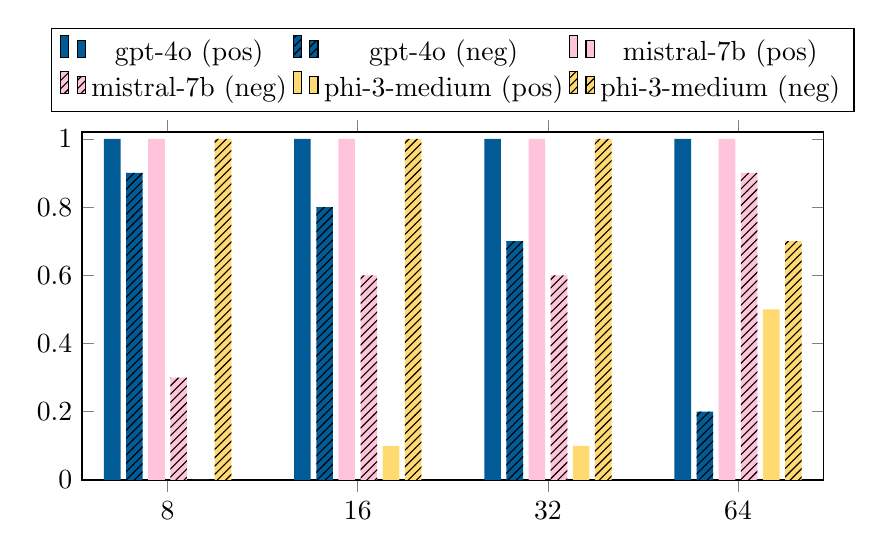
\begin{tikzpicture}
        \begin{axis}[
            ybar,
            bar width=6pt,
            symbolic x coords={8, 16, 32, 64},
            xtick=data,
            ymin=0, ymax=1.02,
            legend columns=3,
            legend style={at={(0.5,1.3)}, anchor=north, draw=black},
            enlarge x limits=0.15,
            width=11cm, height=6cm
        ]
        
        % gpt-4o
        \addplot[fill={rgb,255:red,0;green,91;blue,150}, draw=none] coordinates {(8,1.000) (16,1.000) (32,1.000) (64,1.000)};
        \addlegendentry{gpt-4o (pos)}
        \addplot[fill={rgb,255:red,0;green,91;blue,150}, postaction={
        pattern=north east lines
    }, draw=none] coordinates {(8,0.900) (16,0.800) (32,0.700) (64,0.200)};
        \addlegendentry{gpt-4o (neg)}
        
        % mistral-7b-instruct-v02
        \addplot[fill={rgb,255:red,255;green,196;blue,218}, draw=none] coordinates {(8,1.000) (16,1.000) (32,1.000) (64,1.000)};
        \addlegendentry{mistral-7b (pos)}
        \addplot[fill={rgb,255:red,255;green,196;blue,218}, postaction={
        pattern=north east lines
    }, draw=none] coordinates {(8,0.300) (16,0.600) (32,0.600) (64,0.900)};
        \addlegendentry{mistral-7b (neg)}
        
        % phi-3-medium-128k-instruct
        \addplot[fill={rgb,255:red,255;green,218;blue,112}, draw=none] coordinates {(8,0.000) (16,0.100) (32,0.100) (64,0.500)};
        \addlegendentry{phi-3-medium (pos)}
        \addplot[fill={rgb,255:red,255;green,218;blue,112}, postaction={
        pattern=north east lines
    }, draw=none] coordinates {(8,1.000) (16,1.000) (32,1.000) (64,0.700)};
        \addlegendentry{phi-3-medium (neg)}
        
        \end{axis}
    \end{tikzpicture}}
    \caption{Analysis on \textit{String Search (with subsequence)} across increasing subsequence lengths. This figure examines the behavior of models on \textbf{pos}itive samples (where the subsequence is present) and \textbf{neg}ative samples (where the subsequence is absent).}
    \label{fig:seq_search}
\end{figure}

Figure \ref{fig:seq_search} further analyzes subsequence search performance for GPT-4o, Mistral, and Phi-3-medium. These models exhibit distinct error patterns as the length of the subsequence increases: GPT-4o has no false negative errors (it never misses a present subsequence) but makes more false positive errors as the subsequence length grows, suggesting it overestimates presence in more ambiguous cases.
Mistral also makes no false negative errors but exhibits a decreasing false positive rate, implying it struggles more with shorter distractors. Phi-3-medium, in contrast, makes few false positive errors (rarely identifies an absent sequence as present), but struggles more with false negatives, indicating a general tendency to deny presence. These differing patterns suggest that the models may employ different search strategies, affecting their susceptibility to different types of errors.

For \textit{Batch Search} and \textit{Key-Value Search} tasks (analogous to multi-NIAH and NIAH, respectively), models like Mistral, Phi-3, and Cohere show a notable performance drop, revealing their limitations in handling multiple memory accesses effectively.

% \begin{figure}[h]
%     \centering
%     \begin{subfigure}[t]{0.49\linewidth}
%         \includegraphics[width=\textwidth]{images/recall_black.png}
%         \caption{Black-box models.}
%         \label{fig:first_recall}
%     \end{subfigure}
%     \begin{subfigure}[t]{0.49\linewidth}
%         \includegraphics[width=\textwidth]{images/recall_white.png}
%         \caption{Open-source models.}
%         \label{fig:second_recall}
%     \end{subfigure}
%     \caption{Results for the \textbf{Recall and Edit} tasks.}
%     \label{fig:recall}
% \end{figure}

\begin{figure}[h]
    \centering
    \begin{subfigure}{0.49\columnwidth}
        \resizebox{\textwidth}{!}{
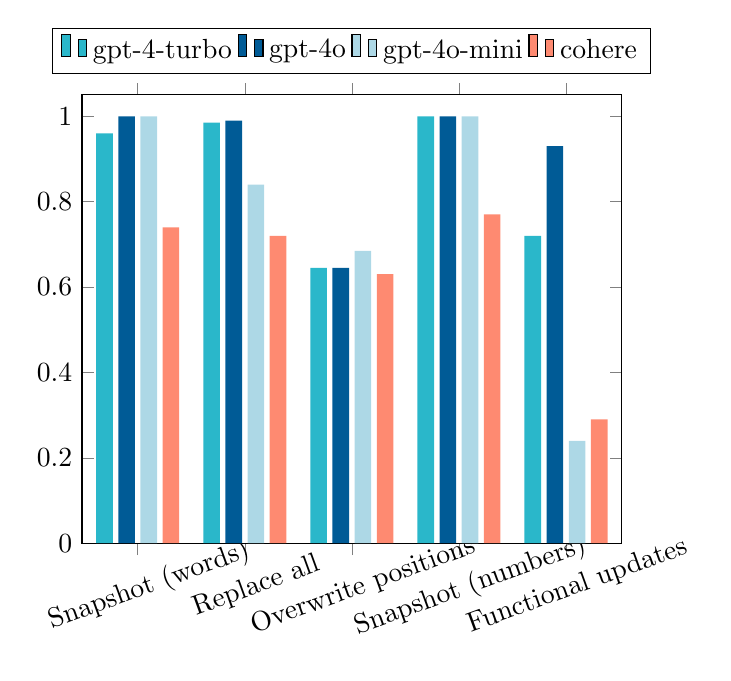
\begin{tikzpicture}
        \begin{axis}[
            ybar,
            bar width=6pt,
            symbolic x coords={Snapshot (words), Replace all, Overwrite positions, Snapshot (numbers), Functional updates},
            xtick=data,
            ymin=0, ymax=1.05,
            legend columns=4,
            legend style={at={(0.5,1.15)}, anchor=north, draw=black},
            enlarge x limits=0.13,
            xticklabel style={rotate=20, anchor=center, yshift=-12pt}
        ]
        
        \addplot[fill={rgb,255:red,42;green,183;blue,202}, draw=none] coordinates {(Snapshot (words),0.96) (Replace all,0.985) (Overwrite positions,0.645) (Snapshot (numbers),1.00) (Functional updates,0.72)};
        \addlegendentry{gpt-4-turbo}
        
        \addplot[fill={rgb,255:red,0;green,91;blue,150}, draw=none] coordinates {(Snapshot (words),1.00) (Replace all,0.99) (Overwrite positions,0.645) (Snapshot (numbers),1.00) (Functional updates,0.93)};
        \addlegendentry{gpt-4o}
        
        \addplot[fill={rgb,255:red,173;green,216;blue,230}, draw=none] coordinates {(Snapshot (words),1.00) (Replace all,0.84) (Overwrite positions,0.685) (Snapshot (numbers),1.00) (Functional updates,0.24)};
        \addlegendentry{gpt-4o-mini}
        
        \addplot[fill={rgb,255:red,254;green,138;blue,113}, draw=none] coordinates {(Snapshot (words),0.74) (Replace all,0.72) (Overwrite positions,0.63) (Snapshot (numbers),0.77) (Functional updates,0.29)};
        \addlegendentry{cohere}
        
        \end{axis}
\end{tikzpicture}}
    \end{subfigure}
    \begin{subfigure}{0.49\columnwidth}
        \resizebox{\textwidth}{!}{    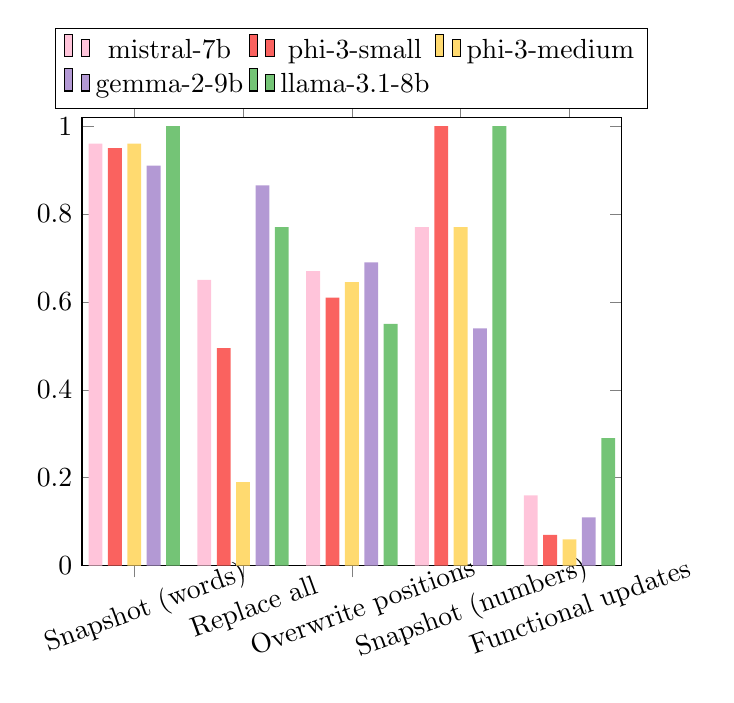
\begin{tikzpicture}
        \begin{axis}[
            ybar,
            bar width=5pt,
            symbolic x coords={Snapshot (words), Replace all, Overwrite positions, Snapshot (numbers), Functional updates},
            xtick=data,
            ymin=0, ymax=1.02,
            legend columns=3,
            legend style={at={(0.5,1.20)}, anchor=north, draw=black},
            enlarge x limits=0.12,
            xticklabel style={rotate=20, anchor=center, yshift=-12pt}
        ]
        
        \addplot[fill={rgb,255:red,255;green,196;blue,218}, draw=none] coordinates {(Snapshot (words),0.96) (Replace all,0.65) (Overwrite positions,0.67) (Snapshot (numbers),0.77) (Functional updates,0.16)};
        \addlegendentry{mistral-7b}
        
        \addplot[fill={rgb,255:red,250;green,98;blue,95}, draw=none] coordinates {(Snapshot (words),0.95) (Replace all,0.495) (Overwrite positions,0.61) (Snapshot (numbers),1.00) (Functional updates,0.07)};
        \addlegendentry{phi-3-small}
        
        \addplot[fill={rgb,255:red,255;green,218;blue,112}, draw=none] coordinates {(Snapshot (words),0.96) (Replace all,0.19) (Overwrite positions,0.645) (Snapshot (numbers),0.77) (Functional updates,0.06)};
        \addlegendentry{phi-3-medium}
        
        \addplot[fill={rgb,255:red,179;green,153;blue,212}, draw=none] coordinates {(Snapshot (words),0.91) (Replace all,0.865) (Overwrite positions,0.69) (Snapshot (numbers),0.54) (Functional updates,0.11)};
        \addlegendentry{gemma-2-9b}
        
        \addplot[fill={rgb,255:red,116;green,196;blue,118}, draw=none] coordinates {(Snapshot (words),1.00) (Replace all,0.77) (Overwrite positions,0.55) (Snapshot (numbers),1.00) (Functional updates,0.29)};
        \addlegendentry{llama-3.1-8b}
        
        \end{axis}
\end{tikzpicture}}
    \end{subfigure}
    \caption{Results for the \textbf{Recall and Edit} tasks.}
    \label{fig:recall}
\end{figure}

\paragraph{Recall and Edit} 
\begin{table}[!h]
    \centering
        \resizebox{0.8\columnwidth}{!}{%
    \begin{tabular}{lllll}
    \toprule
        \textbf{Model} & \textbf{String Search (word)} & \textbf{Snapshot} \\ \hline
gpt-4-turbo    & 1.00 \textcolor{green}{(0.06)} & 1.00 \textcolor{green}{(0.04)} \\ 
gpt-4o         & 1.00 (0.00)                   & 1.00 (0.00)                   \\ 
gpt-4o-mini    & 0.94 \textcolor{red}{(-0.04)}  & 1.00 (0.00)                   \\ 
cohere         & 1.00 (0.00)                   & 1.00 \textcolor{green}{(0.26)} \\ 
mistral-7b     & 1.00 \textcolor{green}{(0.22)} & 0.96 (0.00)                   \\ 
phi-3-small    & 1.00 \textcolor{green}{(0.06)} & 0.99 \textcolor{green}{(0.04)} \\ 
phi-3-medium   & 0.98 \textcolor{red}{(-0.02)}  & 0.87 \textcolor{red}{(-0.09)}  \\ 
gemma-2-9b     & 0.96 \textcolor{red}{(-0.04)}  & 0.96 \textcolor{green}{(0.05)} \\ 
llama-3.1-8b   & 0.98 \textcolor{red}{(-0.02)}  & 1.00 (0.00)                   \\
\bottomrule
    \end{tabular}
    }
    \caption{Ablation study with gibberish context.}
    \label{tab:ablation_gibberish}
\end{table}

Figure \ref{fig:recall} presents the results for the \textbf{Recall and Edit} tasks. While models performed well on basic recall (\textit{Snapshot}), their performance dropped sharply when tasked with making regular edits. A closer analysis of the generated outputs reveals that models struggled with maintaining coherence during edits, often getting trapped in repetitive word loops. For the \textit{Functional Update} task, we deliberately selected simple numerical updates, such as ``Subtract 1 from every number," to ensure the edits were within the models' capabilities. Nevertheless, when comparing performance on \textit{Snapshot (with numbers)} to \textit{Functional Updates}, all models exhibited a steep decline, especially for smaller ones. Analysis of generated outputs revealed that these models frequently deviated from instructions over longer sequences, suggesting difficulties in maintaining consistent rule applications over extended contexts.

Additionally, we conducted a separate ablation study on \textit{Snapshot} and \textit{String Search}. In this study, we replaced meaningful words in the context with gibberish tokens consisting of randomly generated alphabetical characters. As shown in Table \ref{tab:ablation_gibberish}, performance remained largely unchanged, suggesting that semantic meaning was not a significant distractor in these tasks.

\begin{table}
\centering
% \footnotesize
\resizebox{\linewidth}{!}{
\setlength{\tabcolsep}{5pt}
\begin{tabular}[t]{l|ccc}
\toprule
 \makecell[c]{\textbf{Method}} & \makecell[c]{\textbf{Self}\\\textbf{Reflection}} & \makecell[c]{\textbf{Memory}} & \makecell[c]{\textbf{Length}\\\textbf{Generalization}} \\
\midrule
Revision~\cite{DBLP:journals/corr/abs-2408-03314} & \redcross & \greencheck & \redcross \\
Self-Refine~\cite{DBLP:conf/nips/MadaanTGHGW0DPY23} & \greencheck & \greencheck & \redcross \\
Best-of-N~\cite{DBLP:journals/corr/abs-2407-21787} & \redcross & \redcross & \greencheck \\
Beam Search~\cite{ow1988filtered} & \redcross & \redcross & \greencheck \\
Guided Beam Search~\cite{DBLP:conf/nips/XieKZZKHX23} & \greencheck & \redcross & \greencheck \\
\midrule
\textbf{FTTT (ours)} & \greencheck & \greencheck & \greencheck \\
\bottomrule
\end{tabular}
}
% \vspace{-5pt}
\caption{Comparing the advantages and drawbacks of FTTT and related works.}
\label{tab:compare}
% \vspace{-0.5cm}
\end{table}

\begin{table}[!htbp] \centering
  \caption{Human Choices and Predictions About GenAI Choice in the Same Problem: Heterogeneity by Exposure and Attitudes (Pooled)}
\begin{adjustbox}{scale=0.8}
\begin{tabular}{@{\extracolsep{5pt}}lccccc}
% \\[-1.8ex]\hline
% \hline \\[-1.8ex]
\toprule
& \multicolumn{5}{c}{\textit{Dependent variable: Prediction}} \
\cr \cline{2-6}
\\[-1.8ex] & \multicolumn{1}{c}{Heavy User} & \multicolumn{1}{c}{Text-Based LLM User} & \multicolumn{1}{c}{Paid User} & \multicolumn{1}{c}{Agree AI Similar} & \multicolumn{1}{c}{Agree AI Better}  \\
\\[-1.8ex] & (1) & (2) & (3) & (4) & (5) \\
% \hline \\[-1.8ex]
\midrule
 X$\times$Heavy User & -0.056$^{}$ & & & & \\
& (0.052) & & & & \\
 X$\times$Text-Based LLM User & & 0.082$^{**}$ & & & \\
& & (0.040) & & & \\
 X$\times$Paid User & & & -0.001$^{}$ & & \\
& & & (0.072) & & \\
 X$\times$Agree AI Similar & & & & 0.033$^{}$ & \\
& & & & (0.045) & \\
 X$\times$Agree AI Better & & & & & 0.019$^{}$ \\
& & & & & (0.017) \\
 Problem FE & Yes & Yes & Yes & Yes & Yes \\
 X$\times$Problem FE & Yes & Yes & Yes & Yes & Yes \\
 G$\times$Problem FE & Yes & Yes & Yes & Yes & Yes \\
% \hline \\[-1.8ex]
\midrule
 Observations & 2700 & 2700 & 2700 & 2700 & 2700 \\
 % Residual Std. Error & 22.874 & 22.851 & 22.863 & 22.847 & 22.895 \\
% \hline
% \hline \\[-1.8ex]
\bottomrule
\textit{Note:} & \multicolumn{5}{r}{Standard errors are clustered at the problem level. $^{*}$p$<$0.1; $^{**}$p$<$0.05; $^{***}$p$<$0.01} \\
% \multicolumn{6}{r}\textit{} \\
\end{tabular}
\end{adjustbox}
\label{tab:group} \end{table}


\paragraph{Match and Compare}
 As shown in Figure \ref{fig:match}, model performance in the \textbf{Match and Compare} tasks was relatively consistent across different model sizes. Given that counting is a well-known weakness in LLMs, it is unsurprising that all models struggled significantly with the counting task, though GPT models performed slightly better than others. However, models generally succeeded in identifying the duplicates (in \textit{Find duplicates}), and primarily struggled with the counting aspect -- which requires tracking and updating an integer state, a skill that is more similar to stateful processing. This suggests that relying solely on counting-based tests \cite{song2024countingstars} could overly bias the evaluation and fail to capture broader model capabilities. The results also indicate that models exhibit some ability to recognize relative positions and group associations, but their accuracy remains limited (ranging between 0.6-0.8). A closer examination of model generations reveals an overwhelming tendency for the models to produce false positive errors -- models often answer “yes” when the correct answer is “no”, while making very few false negative errors. This means that when the relationship is correct, the models can more reliably identify it. This may stem from a combination of their inherent inclination to agree and the difficulty in recognizing relative comparisons and associations.

% \begin{figure}[h]
%     \centering
%     \includegraphics[width=0.92\columnwidth]{images/difference.png}
%     \caption{Results for \textbf{Spot the Differences }tasks.}
%     \label{fig:difference}
% \end{figure}

\begin{figure}[h]
\centering
\resizebox{0.9\columnwidth}{!}{
 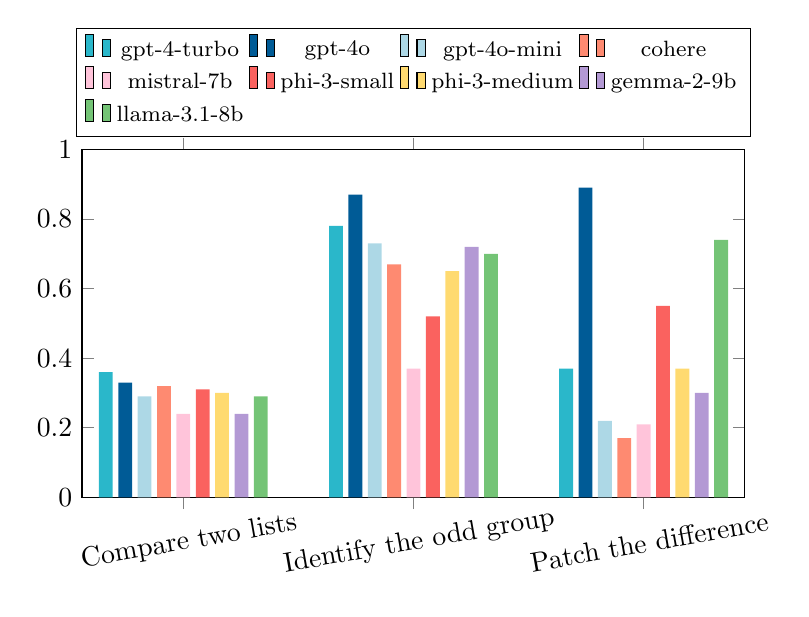
\begin{tikzpicture}
        \begin{axis}[
            ybar,
            bar width=5pt,
            symbolic x coords={Compare two lists, Identify the odd group, Patch the difference},
            xtick=data,
            ymin=0, ymax=1.0,
            legend columns=4,
            legend style={at={(0.5,1.35)}, anchor=north, draw=black, font=\footnotesize},
            enlarge x limits=0.22,
            xticklabel style={rotate=10, anchor=center, yshift=-12pt},
            width=10cm, height=6cm,
        ]
        
        \addplot[fill={rgb,255:red,42;green,183;blue,202}, draw=none] coordinates {(Compare two lists,0.36) (Identify the odd group,0.78) (Patch the difference,0.37)};
        \addlegendentry{gpt-4-turbo}
        
        \addplot[fill={rgb,255:red,0;green,91;blue,150}, draw=none] coordinates {(Compare two lists,0.33) (Identify the odd group,0.87) (Patch the difference,0.89)};
        \addlegendentry{gpt-4o}
        
        \addplot[fill={rgb,255:red,173;green,216;blue,230}, draw=none] coordinates {(Compare two lists,0.29) (Identify the odd group,0.73) (Patch the difference,0.22)};
        \addlegendentry{gpt-4o-mini}
        
        \addplot[fill={rgb,255:red,254;green,138;blue,113}, draw=none] coordinates {(Compare two lists,0.32) (Identify the odd group,0.67) (Patch the difference,0.17)};
        \addlegendentry{cohere}
        
        \addplot[fill={rgb,255:red,255;green,196;blue,218}, draw=none] coordinates {(Compare two lists,0.24) (Identify the odd group,0.37) (Patch the difference,0.21)};
        \addlegendentry{mistral-7b}
        
        \addplot[fill={rgb,255:red,250;green,98;blue,95}, draw=none] coordinates {(Compare two lists,0.31) (Identify the odd group,0.52) (Patch the difference,0.55)};
        \addlegendentry{phi-3-small}
        
        \addplot[fill={rgb,255:red,255;green,218;blue,112}, draw=none] coordinates {(Compare two lists,0.30) (Identify the odd group,0.65) (Patch the difference,0.37)};
        \addlegendentry{phi-3-medium}
        
        \addplot[fill={rgb,255:red,179;green,153;blue,212}, draw=none] coordinates {(Compare two lists,0.24) (Identify the odd group,0.72) (Patch the difference,0.30)};
        \addlegendentry{gemma-2-9b}
        
        \addplot[fill={rgb,255:red,116;green,196;blue,118}, draw=none] coordinates {(Compare two lists,0.29) (Identify the odd group,0.70) (Patch the difference,0.74)};
        \addlegendentry{llama-3.1-8b}
        
        \end{axis}
    \end{tikzpicture}}
    \caption{Results for \textbf{Spot the Differences }tasks.}
    \label{fig:difference}
\end{figure}

\paragraph{Spot the Differences}
As shown in Figure \ref{fig:difference}, performance across all models are poor on \textit{Compare Two Lists}, suggesting inherent difficulties in cross-referencing information across long contexts, even for larger models.  GPT-4o and the LLaMA model significantly outperform the others in the \textit{Identify the Odd Group} task, highlighting a general weakness in detecting contextual differences by the other models. However, an 8B LLaMA model outperforms both equivalently-sized models and even GPT-4 in this task, suggesting that model size alone was not the determining factor. This indicates that architectural differences, training objectives, or specific inductive biases may contribute to improved performance in comparative memory utilization.


\paragraph{Compute on Sets and Lists}
The tasks in this category require models to recognize and process group structures within the context, and performance gradually declines as the complexity of the task increases (see Table \ref{tab:lists}). For instance, in comparing the \textit{Group Membership} task with the \textit{String Search} task, where the former requires identifying which list a word belongs to rather than simply determining its presence, the performance of open-source models drops considerably. Similarly, in comparing the \textit{Group Association} task with the \textit{Group Membership} task, where the former requires determining whether two words belong to the same group, all models exhibit a noticeable decline in performance. The decline becomes even more pronounced when comparing the \textit{ Group Association (alternating)} variant of the task to the standard \textit{Group Association} task. Here, the context involves alternating repeated groups rather than simple group structures, which further challenges the models' abilities to handle partitioned contexts effectively.

An interesting observation was found during the \textit{Iterate} task. In an ablation study, we modified the task to require returning the first words in each list instead of the last words (making it more similar to the \textit{Batch Search} task). The performance sharply declines when models are asked to return the last words, despite their strong information-fetching capabilities. This suggests that, while the models can retrieve information effectively, they struggle to accurately recognize and process partitions within the context.



\begin{table}[t!]
\centering
    \resizebox{0.7\columnwidth}{!}{%

\begin{tabular}{lcc}
\toprule
\textbf{Model} & \textbf{Quantity state} & \textbf{Set state} \\
\midrule
gpt-4-turbo & 0.8 & \textbf{0.80} \\
gpt-4o & \textbf{1.0} & 0.65 \\
gpt-4o-mini & 0.7 & 0.24 \\
cohere & 0.0 & 0.58 \\
mistral-7b & 0.0 & 0.08 \\
phi-3-small & 0.0 & 0.13 \\
phi-3-medium & 0.0 & 0.11 \\
gemma-2-9b & 0.0 & 0.24 \\
llama-3.1-8b & 0.0 & 0.13 \\
\bottomrule
\end{tabular}
}
\caption{Results for \textbf{Stateful Processing} tasks.}
\label{tab:state}
\end{table}
\paragraph{Stateful Processing}

\begin{figure}[t!]
    \centering
    \begin{subfigure}{0.49\columnwidth}
        \resizebox{\textwidth}{!}{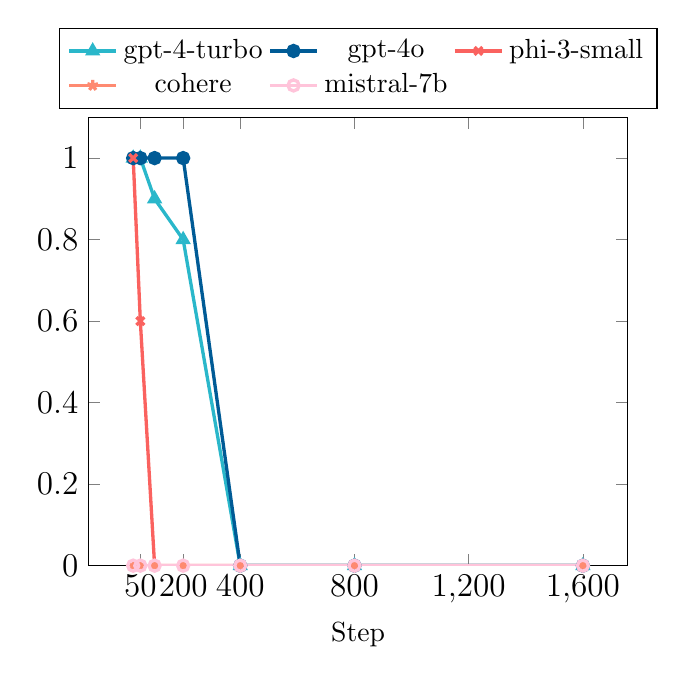
\begin{tikzpicture}
    \begin{axis}[
        xlabel={Step},
        legend style={at={(0.5,1.2)}, anchor=north, cells={align=left}, legend columns=3},
        ymin=0, ymax=1.1,
        xtick={50, 200, 400, 800, 1200, 1600},
        ytick={0,0.2,0.4,0.6,0.8,1.0},
        grid=none,
        tick label style={font=\large}
    ]

    % GPT-4-Turbo
    \addplot[mark=triangle, very thick, color={rgb,255:red,42;green,183;blue,202}] coordinates {
        (25,1.0) (50,1.0) (100,0.9) (200,0.8) (400,0.0) (800,0.0) (1600,0.0)
    };
    \addlegendentry{gpt-4-turbo}

    % GPT-4o
    \addplot[mark=*, very thick, color={rgb,255:red,0;green,91;blue,150}] coordinates {
        (25,1.0) (50,1.0) (100,1.0) (200,1.0) (400,0.0) (800,0.0) (1600,0.0)
    };
    \addlegendentry{gpt-4o}



    % Phi-3-Small
    \addplot[mark=x, very thick, color={rgb,255:red,250;green,98;blue,95}] coordinates {
        (25,1.0) (50,0.6) (100,0.0) (200,0.0) (400,0.0) (800,0.0) (1600,0.0)
    };
    \addlegendentry{phi-3-small}

    % Cohere
    \addplot[mark=star, very thick, color={rgb,255:red,254;green,138;blue,113}] coordinates {
        (25,0.0) (50,0.0) (100,0.0) (200,0.0) (400,0.0) (800,0.0) (1600,0.0)
    };
    \addlegendentry{cohere}

    % Mistral-7B
    \addplot[mark=o, very thick, color={rgb,255:red,255;green,196;blue,218}] coordinates {
        (25,0.0) (50,0.0) (100,0.0) (200,0.0) (400,0.0) (800,0.0) (1600,0.0)
    };
    \addlegendentry{mistral-7b}
    
    \end{axis}
\end{tikzpicture}}
    \end{subfigure}
    \begin{subfigure}{0.49\columnwidth}
        \resizebox{\textwidth}{!}{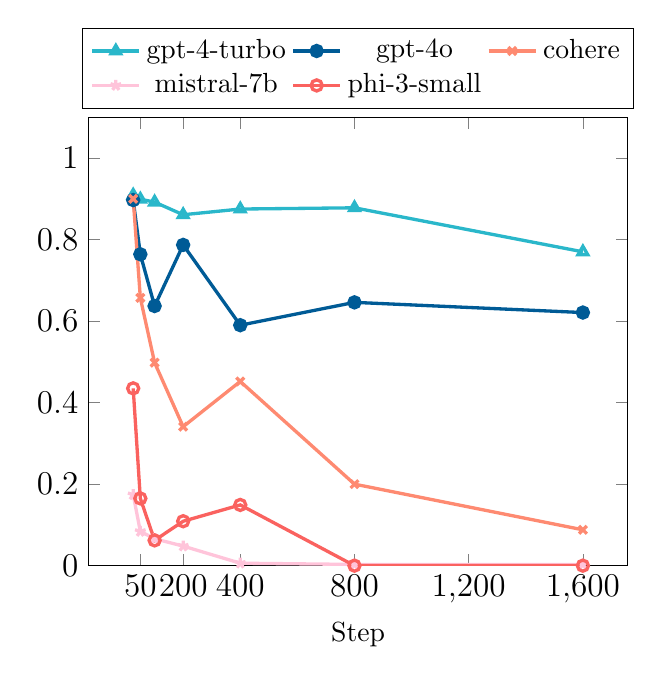
\begin{tikzpicture}
    \begin{axis}[
        xlabel={Step},
        legend style={at={(0.5,1.2)}, anchor=north, cells={align=left}, legend columns=3},
        ymin=0, ymax=1.1,
        xtick={50, 200, 400, 800, 1200, 1600},
        ytick={0,0.2,0.4,0.6,0.8,1.0},
        grid=none,
        tick label style={font=\large}
    ]

    % GPT-4-Turbo
    \addplot[mark=triangle, very thick, color={rgb,255:red,42;green,183;blue,202}] coordinates {
        (25,0.909) (50,0.899) (100,0.892) (200,0.861) (400,0.875) (800,0.878) (1600,0.770)
    };
    \addlegendentry{gpt-4-turbo}

    % GPT-4o
    \addplot[mark=*, very thick, color={rgb,255:red,0;green,91;blue,150}] coordinates {
        (25,0.897) (50,0.764) (100,0.637) (200,0.787) (400,0.590) (800,0.646) (1600,0.621)
    };
    \addlegendentry{gpt-4o}

    % Cohere
    \addplot[mark=x, very thick, color={rgb,255:red,254;green,138;blue,113}] coordinates {
        (25,0.900) (50,0.657) (100,0.498) (200,0.341) (400,0.452) (800,0.200) (1600,0.088)
    };
    \addlegendentry{cohere}

    % Mistral-7B
    \addplot[mark=star, very thick, color={rgb,255:red,255;green,196;blue,218}] coordinates {
        (25,0.174) (50,0.084) (100,0.066) (200,0.048) (400,0.006) (800,0.003) (1600,0.003)
    };
    \addlegendentry{mistral-7b}

    % Phi-3-Small
    \addplot[mark=o, very thick, color={rgb,255:red,250;green,98;blue,95}] coordinates {
        (25,0.435) (50,0.165) (100,0.062) (200,0.109) (400,0.149) (800,0.000) (1600,0.000)
    };
    \addlegendentry{phi-3-small}
    
    \end{axis}
\end{tikzpicture}}
    \end{subfigure}
    \caption{Ablation study on the number of operation steps for the \textbf{quantity state} (left) and\textbf{ set state }(right).}
    \label{fig:ablation_state_step}
\end{figure}



Table \ref{tab:state} presents the results for the \textbf{Stateful Processing} tasks, where performance gaps among models are the most pronounced. The GPT-4(o) models perform well on integer state tracking, while most other models struggle (near zero accuracy). For set state tracking, larger models generally perform better.

We conducted an ablation study to examine how the number of operation steps influences performance of five selected models (Fig. \ref{fig:ablation_state_step}). For quantity state tracking, GPT-4(o) models perform well within fewer than 200 steps but experience a sharp decline in accuracy beyond this threshold. For set state tracking, the performance decline is more gradual. The differences in performance drop between the two tasks can be attributed to the nature of the two tasks. While tracking an integer state might seem simpler than tracking a set, it actually requires the model to maintain and apply every operation sequentially to compute the final value. In contrast, for set state, the fixed size of the set makes more recent operations more relevant to the final state, reducing the need for exhaustive step-by-step tracking. Nevertheless, even in this scenario, all models show a clear inability to handle longer or more complex operation sequences effectively. Interestingly, GPT-4 model outperformed GPT-4o at this task, suggesting potential optimization trade-offs may have affected its ability to manage set-based updates. 

Overall, while larger models like GPT-4(o) exhibit some ability to track state over time, their effectiveness rapidly deteriorates as task complexity increases. Smaller models, in particular, struggle to track operations over time, pointing to significant gaps in their ability to manage and process sequential dependencies critical for state tracking tasks.

\subsection{Results on Composite Tests}

\section{Simple Construction of Projective Compositions}
\label{sec:comp_coord}

It is not clear apriori that projective compositional distributions satisfying Definition \ref{def:proj_comp} ever exist, much less that there is any straightforward way to sample from them.
To explore this, we first restrict attention to perhaps the simplest setting, where the projection functions $\{\Pi_i\}$ are
just coordinate restrictions.
This setting is meant to generalize the intuition we had
in the CLEVR example of Figure~\ref{fig:len_gen},
where different objects were composed in disjoint regions of the image.
We first define the construction of the composed distribution,
and then establish its theoretical properties.








\subsection{Defining the Construction}
Formally, suppose we have a set of distributions
$(p_1, p_2, \ldots, p_k)$ that we wish to compose;
in our running CLEVR example, each $p_i$ is the distribution of images
with a single object at position $i$.
Suppose also we have some reference distribution $p_b$,
which can be arbitrary, but should be thought of as a 
``common background'' to the $p_i$s.
Then, one popular way to construct a composed distribution
is via the \emph{compositional operator} defined below.
(A special case of this construction is used in \citet{du2023reduce}, for example).


\begin{definition}[Composition Operator]
    \label{def:comp_oper}
    Define the \emph{composition operator} $\cC$ acting on an arbitrary set of distributions $(p_b, p_1, p_2, \ldots)$ by
    \begin{align}
    \label{eq:comp_oper}
    \cC[\vec{p}] := \cC[p_b, p_1, p_2, \dots](x) := \frac{1}{Z} p_b(x) \prod_i \frac{p_i(x)}{p_b(x)},
    \end{align}
    where $Z$ is the appropriate normalization constant. We name $\cC[\vec{p}]$ the \emph{composed distribution}, and the score of $\cC[\vec{p}]$ the \emph{compositional score}:
    \begin{align}
    \label{eqn:comp_score}
    &\grad_x \log \cC[\vec{p}](x)  \\
    &= \grad_x \log p_b(x) + \sum_i \left( \grad_x \log p_i(x) - \grad_x \log p_b(x) \right). \notag
    \end{align}
\end{definition}
Notice that if $p_b$ is taken to be the unconditional distribution then this is exactly the Bayes-composition.


\vspace{-0.5em}
\subsection{When does the Composition Operator Work?}
We can always apply the composition operator to any set of distributions,
but when does this actually yield a ``correct'' composition
(according to Definition~\ref{def:proj_comp})?
One special case is when each distribution $p_i$ is
``active'' on a different, non-overlapping set of coordinates.
We formalize this property below
as \emph{Factorized Conditionals} (Definition~\ref{def:factorized}).
The idea is, 
each distribution $p_i$
must have a particular set of ``mask'' coordinates $M_i \subseteq [n]$ which it
samples in a characteristic way,
while independently sampling all other coordinates
from a common background distribution.
If a set of distributions $(p_b, p_1, p_2, \ldots)$ has this
\emph{Factorized Conditional} structure, then 
the composition
operator will produce a projective composition (as we will prove below).



\begin{definition}[Factorized-Conditionals]
\label{def:factorized}

We say a set of distributions $(p_b, p_1, p_2, \dots p_k)$
over $\R^n$
are \emph{Factorized Conditionals} if
there exists a partition of coordinates $[n]$
into disjoint subsets $M_b, M_1, \dots M_k$ such that:
\begin{enumerate}
    \setlength{\itemsep}{1pt}
    \item $(x|_{M_i}, x|_{M_i^c})$ are independent under $p_i$.
    \item $(x|_{M_b}, x|_{M_1}, x|_{M_2}, \dots, x|_{M_k})$
    are mutually independent under $p_b$.
    \item $p_i(x|_{M_i^c}) = p_b(x|_{M_i^c})$.
\end{enumerate}

Equivalently, if we have:
\begin{align}
    p_i(x) &= p_i(x|_{M_i}) p_b(x|_{M_i^c}), \text{ and} \label{eqn:cc-cond}\\
    p_b(x) &= p_b(x|_{M_b}) \prod_{i \in [k]} p_b(x|_{M_i}). \notag
\end{align}
\end{definition}
\vspace{-1em}
Equation~\eqref{eqn:cc-cond} means that each $p_i$
can be sampled by first sampling $x \sim p_b$,
and then overwriting the coordinates of $M_i$
according to some other distribution (which can be specific to distribution $i$).
For instance, the experiment of Figure~\ref{fig:len_gen}
intuitively satisfies this property, since 
each of the conditional distributions could essentially be sampled
by first sampling an empty background image ($p_b$), then ``pasting''
a random object in the appropriate location (corresponding to pixels $M_i$).
If a set of distributions obey this Factorized Conditional structure,
then we can prove that the composition operator $\cC$
yields a correct projective composition,
and reverse-diffusion correctly samples from it.
Below, let $N_t$ denote the noise operator of the
diffusion process\footnote{Our results are agnostic to the specific diffusion noise-schedule and scaling used.} at time $t$.

\begin{theorem}[Correctness of Composition]
\label{lem:compose}
Suppose a set of distributions $(p_b, p_1, p_2, \dots p_k)$
satisfy Definition~\ref{def:factorized},
with corresponding masks $\{M_i\}_i$.
Consider running the reverse-diffusion SDE 
using the following compositional scores at each time $t$:
\begin{align}
s_t(x_t) &:= \grad_x \log \cC[p_b^t, p_1^t, p_2^t, \ldots](x_t),
\end{align}
where $p_i^t := N_t[p_i]$ are the noisy distributions.
Then, the distribution of the generated sample $x_0$ at time $t=0$ is:
\begin{align}
\label{eqn:p_hat}
\hat{p}(x) := p_b(x|_{M_b}) \prod_i p_i(x|_{M_i}).
\end{align}
In particular,
$\hat{p}(x|_{M_i}) = p_i(x|_{M_i})$ for all $i$,
and so
$\hat{p}$ is a projective composition
with respect to projections $\{\Pi_i(x) := x|_{M_i}\}_i$,
per Definition \ref{def:proj_comp}.
\end{theorem}




Unpacking this, Line \ref{eqn:p_hat} says that the final generated distribution
$\hat{p}(x)$ can be sampled by
first sampling
the coordinates $M_b$ according to $p_b$ (marginally),
then independently sampling 
coordinates $M_i$ according to $p_i$ (marginally) for each $i$.
Similarly, by assumption, $p_i(x)$ can be sampled by first sampling the coordinates $M_i$ in some specific way, and then independently sampling the remaining coordinates according to $p_b$. Therefore Theorem \ref{lem:compose} says that $\hat{p}(x)$ samples the coordinates \emph{$M_i$ exactly as they would be sampled by $p_i$}, for each $i$ we wish to compose. 

\begin{proof}(Sketch) \small
Since $\vec{p}$ satisfies Definition \ref{def:factorized}, we have
\begin{align*}
&\cC[\vec{p}](x) := p_b(x) \prod_i \frac{p_i(x)}{p_b(x)} \notag 
= p_b(x) \prod_i \frac{p_b(x_t|_{M_i^c}) p_i(x|_{M_i})}{p_b(x|_{M_i^c})p_b(x|_{M_i})} \notag \\
&= p_b(x) \prod_i \frac{p_i(x|_{M_i})}{p_b(x|_{M_i})} \notag 
= p_b(x|_{M_b}) \prod_i p_i(x_t|_{M_i}) := \hat{p}(x).
\end{align*}
The sampling guarantee follows from the commutativity of composition with the diffusion noising process, i.e. $\cC[\vec{p^t}]= N_t[\cC[\vec{p}]]$. 
The complete proof is in Appendix \ref{app:compose_pf}.
\end{proof}

\begin{remark}
In fact, Theorem~\ref{lem:compose} still holds under any orthogonal transformation of the variables,
because the diffusion noise process commutes with orthogonal transforms.
We formalize this as Lemma~\ref{lem:orthogonal_sampling}.
\end{remark}

\begin{remark}
Compositionality is often thought of in terms of orthogonality between scores.
Definition \ref{def:factorized} implies orthogonality between the score differences that appear in the composed score \eqref{eqn:comp_score}:
$\grad_x \log p_i^t(x_t) - \grad_x \log p_b^t(x_t),$
but the former condition is strictly stronger
(c.f. Appendix \ref{app:score_orthog}).
\end{remark}

\begin{remark}
Notice that the composition operator $\cC$
can be applied to a set of Factorized Conditional
distributions
without knowing the coordinate partition $\{M_i\}$.
That is, we can compose distributions and compute scores
without knowing apriori exactly ``how'' these distributions are supposed to compose
(i.e. which coordinates $p_i$ is active on).
This is already somewhat remarkable, and we will see a much
stronger version of this property in the next section.
\end{remark}

\textbf{Importance of background.}
Our derivations highlight the crucial role of the background
distribution $p_b$ for the composition operator  
(Definition~\ref{def:comp_oper}).
While prior works have taken $p_b$ to be an unconditional distribution and the $p_i$'s its associated conditionals,
our results suggest this is not always the optimal choice -- in particular,
it may not satisfy a Factorized Conditional structure (Definition~\ref{def:factorized}). Figure~\ref{fig:len_gen_monster} demonstrates this empirically: settings (a) and (b) attempt to compose the same distributions using different backgrounds -- empty (a) or unconditional (b) -- with very different results.

\subsection{Approximate Factorized Conditionals in CLEVR.}
\label{sec:clevr-details}

In \cref{fig:len_gen_monster} we explore compositional length-generalization (or lack thereof) in three different setting, two of which (\cref{fig:len_gen_monster}a and \ref{fig:len_gen_monster}c) approximately satisfy \cref{def:factorized}. In this section we explicitly describe how our definition of Factorized Conditionals approximately captures the CLEVR settings of Figures \ref{fig:len_gen_monster}a and \ref{fig:len_gen_monster}c. The setting of \ref{fig:len_gen_monster}b does not satisfy our conditions, as discussed in \cref{sec:problematic-compositions}.

\textbf{Single object distributions with empty background.}
This is the setting of both \cref{fig:len_gen} and \cref{fig:len_gen_monster}a.
The background distribution $p_b$ 
over $n$ pixels is images of an empty scene with no objects.
For each $i \in \{1,\ldots,L\}$ (where $L=4$ in \cref{fig:len_gen} and $L=9$ in \cref{fig:len_gen_monster}a), define the set $M_i \subset [n]$ 
as the set of pixel indices surrounding location $i$.
($M_i$ should be thought of as a ``mask'' that
that masks out objects at location $i$).
Let $M_b := (\cup_i M_i)^c$ be the remaining
pixels in the image.
Then, we claim the distributions $(p_b, p_1, \ldots, p_L)$
form approximately
Factorized Conditionals, with corresponding
coordinate partition $\{M_i\}$.
This is essentially because each distribution $p_i$
matches the background $p_b$ on all pixels except those surrounding
location $i$ (further detail in Appendix~\ref{app:clevr-details}).
Note, however, that the conditions of Definition~\ref{def:factorized}
do not \emph{exactly} hold in the experiment of Figure~\ref{fig:len_gen} -- there is still some dependence between
the masks $M_i$, since objects can cast shadows or even occlude each other.
Empirically, these deviations 
have greater impact
when composing many objects, as seen in \cref{fig:len_gen_monster}a.


\textbf{Bayes composition with cluttered distributions.}
In \cref{fig:len_gen_monster}c we replicate CLEVR experiments in  \citet{du2023reduce, liu2022compositional} where the images contain many objects (1-5) and the conditions label the location of one randomly-chosen object. It turns out the unconditional together with the conditionals can approximately act as Factorized Conditionals in ``cluttered'' settings like this one. The intuition is that if the conditional distributions each contain one specific object plus many independently sampled random objects (``clutter''), then the unconditional distribution \emph{almost} looks like independently sampled random objects, which together with the conditionals \emph{would} satisfy Definition \ref{def:factorized} (further discussion in Appendix \ref{app:clevr-details} and \ref{app:bayes_connect}). This helps to explain the length-generalization observed in \citet{liu2022compositional} and verified in our experiments (\cref{fig:len_gen_monster}c).







\section{Projective Composition in Feature Space}
\label{sec:comp_feature}

\begin{figure}
    \centering
    \includegraphics[width=1.0\linewidth]{figures/feat-space-vis.png}
    \caption{A commutative diagram illustrating Theorem~\ref{lem:transform_comp}.
    Performing composition in pixel space is equivalent 
    to encoding into a feature space ($\cA$),
    composing there,
    and decoding back
    to pixel space ($\cA^{-1}$).
    }
    \label{fig:feat-space-vis}
\end{figure}

So far we have focused on the setting where the projection functions $\Pi_i$ are simply projections onto coordinate subsets $M_i$ in the native space (e.g. pixel space).
This covers simple examples like Figure~\ref{fig:len_gen} but does not include more realistic situations such as Figure~\ref{fig:style-content},
where the properties to be composed are more abstract.
For example a property like ``oil painting'' does not correspond to projection
onto a specific subset of pixels in an image.
However, we may hope that there exists some conceptual feature space
in which ``oil painting'' does correspond to a particular subset of variables.
In this section, we extend our results to the case where the composition occurs in some conceptual feature space, and each distribution to be composed
corresponds to some particular subset of \emph{features}.


Our main result is a featurized analogue of Theorem~\ref{lem:compose}:
if there exists \emph{any} invertible transform $\cA$
mapping into a feature space
where Definition \ref{def:factorized} holds,
then the composition operator (Definition~\ref{def:comp_oper})
yields a projective composition in this feature space, as shown in Figure~\ref{fig:feat-space-vis}.

\begin{theorem}[Feature-space Composition]
\label{lem:transform_comp}
Given distributions $\vec{p} := (p_b, p_1, p_2, \dots p_k)$,
suppose there exists a diffeomorphism $\cA: \R^n \to \R^n$
such that
$(\cA \sharp p_b, \cA \sharp p_1, \dots \cA \sharp p_k)$
satisfy Definition~\ref{def:factorized},
with corresponding partition $M_i \subseteq [n]$.
Then, the composition $\hat{p} := \cC[\vec{p}]$ satisfies:
\begin{align}
\label{eqn:p_hat_A}
\cA \sharp \hat{p}(z)
\equiv
(\cA \sharp p_b (z))|_{M_b} \prod_{i=1}^k (\cA \sharp p_i(z))|_{M_i}.
\end{align}
Therefore, $\hat{p}$
is a projective composition of $\vec{p}$ w.r.t. projection functions
$\{\Pi_i(x) := \cA(x)|_{M_i}\}$.
\end{theorem}
This theorem is remarkable because it means we can
compose distributions $(p_b, p_1, p_2, \dots)$ in the base space,
and this composition will ``work correctly'' in the feature space
automatically (Equation~\ref{eqn:p_hat_A}),
without us ever needing to compute or even know the feature transform $\cA$
explicitly.



Theorem~\ref{lem:transform_comp} may apriori seem too strong
to be true, since it somehow holds for all feature spaces $\cA$
simultaneously.
The key observation underlying Theorem~\ref{lem:transform_comp} 
is that the composition operator $\cC$ behaves
well under reparameterization.
\begin{lemma}[Reparameterization Equivariance]
\label{lem:reparam}
The composition operator of Definition~\ref{def:comp_oper}
is reparameterization-equivariant. That is,
for all diffeomorphisms $\cA: \R^n \to \R^n$
and all tuples of distributions $\vec{p} = (p_b, p_1, p_2, \dots, p_k)$,
\begin{align}
 \cC[ \cA \sharp \vec{p}] =  \cA \sharp \cC[\vec{p}].
\end{align}
\end{lemma}
\arxiv{\footnote{
For example (separate from our goals in this paper):
Classifier-Free-Guidance can be seen as an instance of the composition operator.
Thus, Lemma~\ref{lem:reparam} implies that performing CFG
in latent space is \emph{equivalent} to CFG in pixel-space,
assuming accurate score-models in both cases.}}
\arxiv{This lemma is potentially of independent interest:
reparametrization-equivariance
is a very strong property which is typically not satisfied by
standard operations between probability distributions---
for example, the ``simple product'' $p_1(x)p_2(x)$ does not satisfy it---
so it is mathematically notable that the composition operator 
has this structure.
Lemma~\ref{lem:reparam} and Theorem~\ref{lem:transform_comp}
are proved in Appendix \ref{app:param-indep}.}

This lemma is potentially of independent interest:
equivariance distinguishes the composition operator
from many other common operators
(e.g. the simple product).
Lemma ~\ref{lem:reparam} and Theorem~\ref{lem:transform_comp}
are proved in Appendix \ref{app:param-indep}.

\section{Sampling from Compositions.}
The feature-space Theorem~\ref{lem:transform_comp} is weaker than Theorem~\ref{lem:compose}
in one important way: it does not provide a sampling algorithm.
That is, Theorem~\ref{lem:transform_comp} guarantees that $\hat{p} := \cC[\vec{p}]$
is a projective composition, but does not guarantee that reverse-diffusion
is a valid sampling method.

There is one special case where diffusion sampling \emph{is} guaranteed to work, namely, for orthogonal transforms (which can seen as a straightforward extension of the coordinate-aligned case of \cref{lem:compose}):
\begin{lemma}[Orthogonal transform enables diffusion sampling]
\label{lem:orthogonal_sampling}
If the assumptions of Lemma \ref{lem:transform_comp} hold for $\cA(x) = Ax$, where $A$ is an orthogonal matrix, then running a reverse diffusion sampler with scores $s_t = \grad_x \log \cC[\vec{p}^t]$ generates the composed distribution $\hat{p} = \cC[\vec{p}]$ satisfying \eqref{eqn:p_hat_A}.
\end{lemma}
The proof is given in \cref{app:orthog_sample_pf}.

However, for general invertible transforms, we have no such sampling guarantees.
Part of this is inherent: in the feature-space setting, the 
diffusion noise operator $N_t$ no longer commutes
with the composition operator $\cC$ in general,
 so scores of the noisy composed 
distribution $N_t[\cC[\vec{p}]]$
cannot be computed from scores
of the noisy base distributions $N_t[\vec{p}]$.
Nevertheless, one may hope to sample from the distribution $\hat{p}$
using other samplers besides diffusion, 
such as annealed Langevin Dynamics
or
Predictor-Corrector methods \citep{song2020score}.
We find that the situation is surprisingly subtle:
composition $\cC$ produces distributions which
are in some cases easy to sample (e.g. with diffusion),
yet in other cases apparently hard to sample.
For example, in the
setting of Figure~\ref{fig:clevr_color_comp}, 
our Theorem~\ref{lem:transform_comp} implies
that all pairs of colors should compose equally well
at time $t=0$, since there exist diffeomorphisms
(indeed, linear transforms) between different colors.
However, as we saw,
the diffusion sampler
fails to sample from compositions 
of non-orthogonal colors--- and 
empirically, even more sophisticated
samplers such as Predictor-Correctors
also fail in this setting.
At first glance, it may seem odd that
composed distributions are so hard to sample,
when their constituent distributions are relatively easy to sample.
One possible reason for this below is that the composition operator has extremely poor Lipchitz constant,
so it is possible for a set of distributions $\vec{p}$ to ``vary smoothly''
(e.g. diffusing over time) while their composition $\cC[\vec{p}]$
changes abruptly.
We formalize this in \cref{lem:lipschitz} (further discussion and proof in Appendix \ref{app:lipschitz}).
\begin{lemma}[Composition Non-Smoothness]
\label{lem:lipschitz}
For any set of distributions $\{p_b, p_1, p_2, \dots, p_k\}$,
and any noise scale $t := \sigma$,
define the noisy distributions 
$p_i^t := N_{t}[p_i]$,
and let $q^t$ denote the composed distribution at time $t$: $q^t := \cC[\vec{p}^t]$. Then, for any choice of $\tau > 0$,
there exist distributions $\{p_b, p_1, \dots p_k\}$ over $\R^n$
such that
\begin{enumerate}
    \setlength{\itemsep}{0pt}
    \item For all $i$, the annealing path of $p_i$ is 
    $\cO(1)$-Lipshitz:
    $\forall t, t': W_2(p_i^{t}, p_i^{t'}) \leq \cO(1) |t - t'|$.
    \item The annealing path of $q$ has Lipshitz constant
    at least $\Omega(\tau^{-1})$:
    $\exists t, t': W_2(q^{t}, q^{t'}) \geq \frac{|t - t'|}{2\tau}.$
\end{enumerate}
\end{lemma}




The composite tests significantly challenge the models by combining multiple atomic capabilities into a single test. In the \textit{Processing Data Blocks} task, the context is fixed at 4k tokens, while for the \textit{Theory of Mind} task, the number of operation steps is set to 100. As shown in Table \ref{tab:comp}, model performance on both tasks are generally low, showing a broad inability to handle the more complex scenarios. Performance across all models drop substantially on composite tasks compared to their performance on individual capability tasks, such as search, recall, and group processing. 

Interestingly, some smaller models, like Mistral and Phi-3-small, exhibit slightly better performance on the \textit{Theory of Mind} task than on the set state tracking task. This anomaly likely stems from their already weak state tracking ability, which limits their performance across both tasks. Additionally, these models tend to generate longer answers in the set state task which reduces the set overlap.

Notably, even the most capable models, such as GPT-4-turbo and GPT-4o, struggle, showing that scaling model size alone is not enough for solving these composite tasks. Additionally, the variation in performance among smaller models suggests that their limitations stem not only from size but also from underlying architectural or training differences. This indicates that smaller models require more targeted care to bridge the gap in effective memory use.



\section{Related Work}
\label{sec:related_work}

The original investigation \cite{gibson1979ecological} on the relationship between visual perception and human action defines \emph{affordance} as the opportunities for interaction with the surrounding environment. Behavioral studies on regular and cognitively impaired persons have shown evidence that perception results in both visual and motor signals in the human brain. An extended study \cite{anderson2002attentional} shows that visual attention to the spatial characteristics of the perceived objects initiates automatic motor signals for different actions. In computer vision, human affordance learning involves novel pose prediction such that the estimated pose represents a valid human action within the scene context. The task is fundamental to many problems requiring robust semantic reasoning about the environment, such as human motion synthesis \cite{wang2021scene} and scene-aware human pose generation \cite{wang2017binge, roy2016multi, zhang2022inpaint, yao2023scene}.

Earlier methods of affordance learning have explored knowledge mining \cite{zhu2014reasoning} and multimodal feature cues \cite{roy2016multi} to address the problem. In \cite{zhu2014reasoning}, the authors use a Markov Logic Network for constructing a knowledge base by extracting several object attributes from different image and metadata sources, which can perform various downstream visual inference tasks without any additional classifier, including zero-shot affordance prediction. In \cite{roy2016multi}, the authors use depth map, surface normals, and segmentation map as multimodal cues to train a multi-scale convolutional neural network (CNN) for scene-level semantic label assignment associated with specific human actions. In \cite{do2018affordancenet}, the authors design a multi-branch end-to-end CNN with two separate pathways for object detection and affordance label assignment to achieve high real-time inference throughput. Researchers \cite{chuang2018learning} have also explored socially imposed constraints for affordance learning. In \cite{chuang2018learning}, the authors propose a graph neural network (GNN) to propagate contextual scene information from egocentric views for action-object affordance reasoning.

Probabilistic modeling of scene-aware human motion generation also involves semantic reasoning of human interaction with the environment. Initial works on human motion synthesis have taken different architectural approaches, such as sequence-to-sequence models \cite{barsoum2018hp}, generative adversarial networks (GAN) \cite{barsoum2018hp, cai2018deep, yang2018pose}, graph convolutional networks (GCN) \cite{yan2019convolutional}, and variational autoencoders (VAE) \cite{guo2020action2motion}. However, these methods have mostly ignored the role of environmental semantics. Due to potential uncertainty in human motion, in a recent approach \cite{wang2021scene}, the authors address such motion synthesis with a GAN conditioned on scene attributes and motion trajectory to predict probable body pose dynamics.

One key challenge of human affordance generation in 2D scenes is the lack of large-scale datasets with rich pose annotations. In \cite{wang2017binge}, the authors compile the only public dataset of annotated human body poses in complex 2D indoor scenes by extracting frames from sitcom videos. Aiming to generate a contextually valid human affordance at a user-defined location, the authors propose sampling the scale and deformation parameters for an existing human pose template using a VAE conditioned on the localized image patches as scene context. In \cite{zhang2022inpaint}, the authors introduce a two-stage GAN architecture for achieving a similar goal by estimating the affine bounding box parameters to localize a probable human in the scene and then generating a potential body pose at that location. The method uses the input scene, corresponding depth, and segmentation maps as semantic guidance. In \cite{yao2023scene}, the authors propose a transformer-based approach with knowledge distillation for generating human affordances in 2D indoor scenes.


\section{Conclusion}

%In this paper, w
We propose a new PEFT method called DiffoRA, which enables efficient and adaptive LLM fine-tuning based on LoRA. 
Instead of adjusting every interior rank, 
%of the decomposition matrices 
%of all modules, 
we argue that adopting LoRA module-wisely is sufficient. 
To achieve this, we construct a DAM to select the modules that are most suitable and essential to fine-tune. We theoretically analyze how the DAM impacts the convergence rate and generalization capability.
%of the pre-trained model. 
Furthermore, we adopt continuous relaxation and discretization to establish DAM.
%for each task. 
To alleviate the issue of discretization discrepancy, we utilize the weight-sharing strategy for optimization. 
%We fully implement our method and t
The experimental results demonstrate that our DiffoRA works consistently better than the baselines across all benchmarks. 


% \section*{Impact Statement}

% This paper contributes to the advancement of Machine Learning by introducing a systematic and programmable evaluation framework for assessing the contextual processing capabilities of large language models. Our work provides insights into model strengths and limitations in handling various atomic and composite tasks, offering a structured way to analyze model behavior. These contributions can guide future research in improving model efficiency and reliability.

% We do not foresee any direct ethical concerns or negative societal consequences arising from this work. Our evaluation methodology is designed to be model-agnostic and does not involve sensitive data or high-stakes applications.


% In the unusual situation where you want a paper to appear in the
% references without citing it in the main text, use \nocite
\nocite{langley00}

\bibliography{references}
\bibliographystyle{icml2025}


%%%%%%%%%%%%%%%%%%%%%%%%%%%%%%%%%%%%%%%%%%%%%%%%%%%%%%%%%%%%%%%%%%%%%%%%%%%%%%%
%%%%%%%%%%%%%%%%%%%%%%%%%%%%%%%%%%%%%%%%%%%%%%%%%%%%%%%%%%%%%%%%%%%%%%%%%%%%%%%
% APPENDIX
%%%%%%%%%%%%%%%%%%%%%%%%%%%%%%%%%%%%%%%%%%%%%%%%%%%%%%%%%%%%%%%%%%%%%%%%%%%%%%%
%%%%%%%%%%%%%%%%%%%%%%%%%%%%%%%%%%%%%%%%%%%%%%%%%%%%%%%%%%%%%%%%%%%%%%%%%%%%%%%
\newpage
\appendix
\onecolumn
\section{Test Templates}
\label{apd:prompt_example}
In this appendix, we provide the templates of the test prompts. Placeholder context words such as "aaa, bbb, ccc," etc., are used for illustration purposes. During testing, these context words are uniformly sampled from an English dictionary. Variable tokens in the instruction part are marked with the \textbf{bold} font.

\begin{longtable}{p{3cm}p{12cm}}
        \toprule
        \multicolumn{2}{c}{\textbf{Search} } \\
        \midrule
         Task name & Prompt  \\
         \midrule
         String search (with word) & \textit{Context:}
         
         aaa, bbb, ccc, ...
         
         \textit{Instruction:}
         
         Given the context, determine if the word ``\textbf{bbb}" is present in the context. Answer with ``yes'' or `no''.
         
         Answer: \\
         
         \midrule
         String search (with subsequence) & \textit{Context:}
         
         aaa, bbb, ccc, ...
         
         \textit{Instruction:}
         
         Given the list of words in the context, determine if the sequence ``\textbf{bbb, xxx, ddd}'' appears in the context. Answer with 'yes' or 'no'.
         
         Answer: \\
         
         \midrule
         
         Key-value search & \textit{Context:} 
         
         aaa:bbb, ccc:ddd, ...
         
         \textit{Instruction:}
         
         Given a list of word pairs formatted as ``word\_1: word\_2'' in the context, return the second word associated with the provided first word. For the first word ``\textbf{aaa}'', the corresponding second word is:\\
         \midrule
         Batch search & \textit{Context: }
         
         aaa:bbb, ccc:ddd, ...
         
        \textit{Instruction:}
         
         Given a list of word pairs formatted as ``word\_1: word\_2'' in the context, return the second word associated with the provided first words. For the first words: \textbf{aaa, ccc, ...}, the corresponding second words are:\\
        \bottomrule
        \toprule
        
        \multicolumn{2}{c}{\textbf{Recall and Edit} } \\
        \midrule
         Task name & Prompt  \\
        \midrule
        Snapshot & \textit{Context:}
        
        aaa, bbb, ccc, ...
        
        \textit{Instruction:}
        
        Repeat the previous context exactly as it is, without making any additions or deletions.
        
        Answer:\\
        \midrule

        Replace all (x to y) & \textit{Context:}

        aaa, bbb, aaa, ccc, aaa, ddd, ...

        \textit{Instruction:}
        
        Repeat the previous context and replace the word ``\textbf{aaa}'' with ``\textbf{zzz}'' each time it appears.
        
        Answer: \\
        \midrule
        Replace all (x to null) & \textit{Context:}

        aaa, bbb, aaa, ccc, aaa, ddd, ...

        \textit{Instruction:}
        
        Repeat the previous context but skip the word ``\textbf{aaa}'' each time it appears.
        
        Answer: \\
        \midrule
        Overwrite positions (nth to y) & \textit{Context:}

        aaa, bbb, ccc, ...
        
        \textit{Instruction}:
        
        Repeat the previous context and replace every \textbf{third} word with ``zzz''.
        
        Answer: \\
        \midrule
        Overwrite positions (nth to null) & \textit{Context:}

        aaa, bbb, ccc, ...
        
        \textit{Instruction}:
        
        Repeat the previous context and skip every \textbf{other} word.
        
        Answer: \\
        \midrule

        Functional updates & \textit{Context:}

        111, 222, 333, ...
        
        
        \textit{Instruction:}
        
        \textbf{Add 3} to every number in the previous context.
        
        Answer: \\
        \bottomrule
        \toprule
        \multicolumn{2}{c}{\textbf{Match and Compare} } \\
        \midrule
         Task name & Prompt  \\
        \midrule

        Compare positions & \textit{Context}:
        
        aaa, bbb, ccc, ...
        
        \textit{Instruction}:
        
        Given the list of words in the context, determine the relative positions of two words. Does the word ``\textbf{aaa}'' appear before the word ``\textbf{ccc}'' in the list? Answer ``yes'' or ``no''.
        
        Answer: \\

        \midrule

        Find duplicates & \textit{Context}:
        
        aaa, bbb, aaa, ...
        
        \textit{Instruction}:
        
        A word is repeated multiple times in the context. Your task is to identify the word that is repeated.
        
        The repeated word is: \\

        \midrule

        Count & \textit{Context}:
        
        aaa, bbb, aaa, ...
        
        \textit{Instruction}: 
        
        Count the number of times the word ``\textbf{aaa}'' appeared in the context.
        
        Answer: The word ``\textbf{aaa}'' appeared \\

         \midrule

        Check association & \textit{Context}:
               
        aaa:attribute 1, bbb:attribute 2, ccc: attribute 2, ddd: attribute 1, ...

        \textit{Instruction}:

        Given the list of words and their respective attributes in the format of ``word:attribute'', determine if the word ``\textbf{aaa}'' and the word ``\textbf{ggg}'' have the same attribute. Answer with ``yes'' or ``no''.

        Answer: \\

        \bottomrule
        \toprule
        \multicolumn{2}{c}{\textbf{Spot the Differences} } \\
        \midrule
         Task name & Prompt  \\
        \midrule

        Compare two lists & \textit{Context}:
        
        List 1: aaa, bbb, ccc, ...
        
        List 2: aaa, ddd, ccc, ...
        
        \textit{Instruction}: 
        
        There are two lists of words in the context. The first list contains the original words. The second list is similar to the first but has some words replaced with different ones. Your task is to identify the words in the \textbf{first/second} list that are different from those in the other list. Provide the different words as your answer.
        
        Answer: \\

        \midrule

        Identify the odd group & \textit{Context}:
        
        List 1: aaa, bbb, ccc, ...
        
        List 2: bbb, aaa, ccc, ...
        
        List 3: aaa, zzz, ccc, ...
        
        List 4: ccc, aaa, bbb, ...
        
        \textit{Instruction}:
        
        Given the lists of words in the context, identify the list that is different from the others. Provide the list number as your answer. For example, if the Nth list is different, provide "List N" as your answer.
        
        Answer: \\
        \midrule
        Patch the difference & \textit{Context}:
        
        aaa, bbb, ccc, aaa, bbb, ccc, ...
        
        \textit{Instruction}: 
        
        Given the sequence of words that follows a specific pattern in the context, predict the \textbf{Nth} word that appears after the final word in the given sequence.
        
        Answer: The \textbf{Nth} word that appears after the final word in the given sequence is\\

        \bottomrule
        \toprule

        \multicolumn{2}{c}{\textbf{Compute on Sets and Lists} } \\
        \midrule
         Task name & Prompt  \\
        \midrule

        Group membership & \textit{Context}:
        
        List 1: aaa, bbb, ccc, ...\newline
        List 2: ddd, eee, fff, ...\newline
        ...
        
        \textit{Instruction}:
        
        Given the lists of words in the context, determine which list contains the word ``\textbf{fff}". If the word is not present in either list, answer ``no".
        
        Answer:\\

       
        \midrule
        Group association & \textit{Context}:
        
        List 1: aaa, bbb, ccc, ...\newline
        List 2: ddd, eee, fff, ...\newline
        ...
        
        \textit{Instruction}:
        
        Given the lists of words in the context, determine if the word ``\textbf{aaa}'' and the word ``\textbf{eee}'' are in the same list. Answer with ``yes'' or ``no''.

        Answer: \\
        \midrule

        Group association (alternating) & Context:

        Role A: aaa, bbb, ...\newline
        Role B: ccc, ddd, ...\newline
        Role A: eee, fff, ...\newline
        Role B: ggg, hhh, ...\newline
        ...

        Instruction:

        Given the context with alternating roles and their respective context words, determine if the word ``\textbf{aaa}'' and the word ``\textbf{ggg}'' are in the same role. Answer with ``yes'' or ``no''.

        Answer:\\

        \midrule
        Iterate & \textit{Context}:
        
        List 1: aaa, bbb, ccc, ...\newline
        List 2: ddd, eee, fff, ...\newline
        ...
        
        \textit{Instruction}:
        
        Given the lists of words in the context, identify and recall the \textbf{last} word from each list. Provide your answer as a list of these words separated by commas. \\
        & Answer:
        \\
 
        \bottomrule
        \toprule

        \multicolumn{2}{c}{\textbf{Stateful Processing} } \\
        \midrule
         Task name & Prompt  \\

        \midrule
        Quantity state & \textit{Context}:
        
        Begin with the number xx. Perform the following operations:\newline
        1. Add xx
        2. Subtract xx
        3. ...
    
        \textit{Instruction}:
        
        In the context, you are given an initial number and a series of operations to perform on that number. Your task is to determine the final result of the operations. Write your final answer after the text "FINAL ANSWER:". For example, "FINAL ANSWER: 42".
        
        FINAL ANSWER:\\ 
        \midrule
        Quantity & \textit{Agent actions}:
        
        Agent draws aaa, bbb, ccc\newline
        Agent discards bbb, ccc\newline
        Agent draws ddd, fff\newline
        Agent discards ddd\newline
        ...

        \textit{Instruction}:
        
        Given the actions of the agent, your task is to determine the final list of words the agent ends up with after a series of actions. Write your final answer after the text ``FINAL ANSWER:". For example, ``FINAL ANSWER: word1, word2, word3".
        
        FINAL ANSWER:\\
       
        \bottomrule

        \toprule
        \multicolumn{2}{c}{\textbf{Processing Data Blocks} } \\
        \midrule
         Task name & Prompt  \\
        \midrule
        Processing Data Blocks & \textit{Context}:
        
        Role 1: aaa, bbb, ccc, ...\newline
        Role 2: ddd, eee, fff, ...\newline
        Role 3: ggg, hhh, iii, ... \newline
        Role 1: jjj, kkk, ... \newline
        ...
        
        \textit{Instruction}:
        
        The context consists of a series of alternating roles, each associated with a list of words. Your task is to identify and recall all the words from the role labeled ``{\textbf{Role 2}}" that appear after the word ``{\textbf{zzz}}" in the sequence. Please write your answer after the text ``Answer:". For example, ``Answer: word1, word2, word3".
        
        Answer:\\
        \bottomrule
        \toprule
        \multicolumn{2}{c}{\textbf{Composite-State Tracking (Theory of Mind)} } \\
        \midrule
         Task name & Prompt  \\
        \midrule
        Theory of Mind & \textit{Agents actions:}:
        
        Agent A starts with the following words: aaa, bbb, ccc, ...\newline
        Agent B starts with the following words: ddd, eee, fff, ...\newline
        Agent B starts with the following words: ggg, hhh, iii, ...\newline
        Agent B swaps the following words ``ddd" with Agent C for the following words ``hhh". \newline
        Agent A discards the following words: ccc, zzz, .... \newline
        Agent C draws the following words: xxx, yyy, .... \newline
        ...
        
        \textit{Instruction}:
        
        Given the actions of the agents, your task is to determine the final list of words each agent ends up with after a series of actions. Write your final answer after the text "FINAL ANSWER:". For example, "FINAL ANSWER: Agent A: word1, word2, word3\textbackslash nAgent B: word4, word5".
        
        FINAL ANSWER:\\
        \bottomrule
        
    \label{tab:level1}
\end{longtable}



\section{Task Details}
\label{apd:task_detail}

This appendix provides details for each task, including the number of examples, evaluation metrics, and configurable hyperparameters. The context length is fixed at 4k for almost all tasks, apart from Stateful Processing, where the context is determined by number of operation steps and set to 200 for quantity state and 100 for set state, which maps to around 1.5k context tokens.

Here is an example of number of examples calculation String search (with word):  5 (query depth) *  2 (labels)  * 5 (samples per parameter setting) = 50. 


\begin{longtable}{lp{6.5cm}cc}
\caption{Task Overview with Hyperparameters, Number of Examples, and Evaluation Metrics\label{tab:task_details}} \\

\toprule
\textbf{Task Name} & \textbf{Hyperparameters} & \textbf{\# of Examples} & \textbf{Metric} \\ 
\midrule
\endfirsthead

\toprule
\textbf{Task Name} & \textbf{Hyperparameters} & \textbf{\# of Examples} & \textbf{Metric} \\ 
\midrule
\endhead

\midrule
\multicolumn{4}{r}{\textbf{Continued on next page}} \\ 
\midrule
\endfoot

\bottomrule
\endlastfoot

\multicolumn{4}{l}{\textbf{Search}} \\ 
String search (word) & query depth = [0, 0.25, 0.5, 0.75, 1], label = [positive, negative], samples = 5 & 50 & exact\_match \\
String search (sequence) & sequence length = [8, 16, 32, 64], label = [positive, negative], samples = 10 & 80 & exact\_match \\ 
Key-value search & query depth = [0, 0.25, 0.5, 0.75, 1], samples = 10 & 50 & exact\_match \\ 
Batch search & batch size = [4, 8, 16, 32], samples = 5 & 20 & rouge-L\_recall \\
\midrule
\multicolumn{4}{r}{\textbf{Number of Entries for Category: 200}} \\ 
\midrule

\multicolumn{4}{l}{\textbf{Recall and Edit}} \\ 
Snapshot (words) & samples = 10 & 10 & rouge-L \\
Replace all & density = [0.2, 0.4, 0.6, 0.8], y = [random word, null], samples = 5 & 40 & rouge-L \\
Overwrite positions & nth = [2, 3, 4], y = [random word, null], samples = 5 & 30 & rouge-L \\ 
Snapshot (numbers) & samples = 10 & 10 & rouge-L \\ 
Functional updates & function type = [add (3), subtract (1), multiply (2)], samples = 5 & 15 & rouge-L \\ 
\midrule
\multicolumn{4}{r}{\textbf{Number of Entries for Category: 105}} \\ 
\midrule

\multicolumn{4}{l}{\textbf{Match and Compare}} \\ 
Compare positions & query 1 depth = [0, 0.25, 0.5, 0.75, 1], query 2 depth = [0, 0.25, 0.5, 0.75, 1], samples = 3 & 75 & exact\_match \\ 
Find duplicates & repetition = [2, 4, 8, 16, 32], samples = 5 & 25 & exact\_match \\ 
Count & repetition = [2, 4, 8, 16, 32], samples = 5 & 25 & exact\_match \\ 
Check association & n attribute = [2, 4, 8, 16, 32], label = [positive, negative], samples = 5 & 50 & exact\_match \\
\midrule
\multicolumn{4}{r}{\textbf{Number of Entries for Category: 175}} \\ 
\midrule

\multicolumn{4}{l}{\textbf{Spot the Differences}} \\ 
Compare two lists & num different words = [1, 5, 10, 20], chosen list = [first, second], samples = 10 & 80 & rouge-L\_recall \\ 
Identify the odd group & words per group = [25, 50, 75, 100], percentage of difference = [0, 0.25, 0.5], samples = 5 & 60 & exact\_match \\ 
Patch the difference & pattern length = [2, 15, 30],  cut off depth = [0, 0.5, 1], nth = [1, 3, 6], samples = 5 & 120\footnote{For \textit{Patch the difference} task with pattern length 2, there is only two cut off percentage options; therefore the total number of data points is 120 instead of 135.} & exact\_match \\ 
\midrule
\multicolumn{4}{r}{\textbf{Number of Entries for Category: 260}} \\ 
\midrule

\multicolumn{4}{l}{\textbf{Compute on Sets and Lists}} \\ 
Group membership & number of groups = [4, 8, 16, 32], query depth = [0, 0.25, 0.5, 0.75, 1], samples = 5 & 100 & exact\_match \\ 
Group association & number of groups = [4, 8, 16, 32], label = [positive, negative], samples = 5  & 40 & exact\_match \\ 
Group association (alternating) & number of groups = [2, 4, 8, 16, 32], number of turns = 10, label = [positive, negative], sample = 5 & 50 & exact\_match \\
Iterate & number of groups = [4, 8, 16, 32], samples = 5 & 20 & rouge-L \\ 
\midrule
\multicolumn{4}{r}{\textbf{Number of Entries for Category: 210}} \\ 
\midrule

\multicolumn{4}{l}{\textbf{Stateful Processing}} \\ 
Set state & number of steps = 100, set size = [5, 10, 15, 20], samples = 10 & 40 & jaccard\_similarity \\ 
Quantity state & number of steps = 200, samples = 10 & 10 & exact\_match \\ 
\midrule
\multicolumn{4}{r}{\textbf{Number of Entries for Category: 50}} \\ 
\midrule

\multicolumn{4}{l}{\textbf{Composite}} \\ 
Composite edits of data blocks & number of blocks = [2, 4, 8, 16, 32], number of turns = 10, samples = 5 & 50 & rouge-L \\
Theory of mind & number of steps = 100, number of agents = [2, 3, 4], samples = [10, 20] & 60 & jaccard\_similarity \\ 
\midrule
\multicolumn{4}{r}{\textbf{Number of Entries for Category: 110}} \\ 
\midrule

\multicolumn{4}{r}{\textbf{Total Number of Entries: 1110}} \\ 
\end{longtable}



\section{Evaluation Metrics}
\label{apd:eval}
In this appendix section, we provide details about the evaluation metrics we have used in the tests.

\begin{itemize} \item Exact Match: The exact match accuracy measures whether the generated answer exactly matches the reference answer. It is computed as follows: 
\[
\text{Exact Match} = 
\begin{cases} 
1 & \text{if } \text{reference\_answer} = \text{generated\_answer}, \\
0 & \text{otherwise}.
\end{cases}
\]
\item ROUGE-L / ROUGE-L-recall: ROUGE (Recall-Oriented Understudy for Gisting Evaluation) \cite{lin-2004-rouge} measures the verbatim overlap between the reference and the generated answers. ROUGE-L specifically looks for the longest common subsequence (LCS) between the two texts, which reflects the structure of the text and the longest sequence of matching words. ROUGE-L recall focuses on the ability of the model to recall the content from the reference answer, and it emphasizes matching the longest subsequences.

ROUGE-L-recall can be defined as:
\[
\text{ROUGE-L-recall} = \frac{LCS(\text{generated\_answer}, \text{reference\_answer})}{\text{length of reference\_answer}}
\]

ROUGE-L is computed as the F1-score, which combines both precision and recall to provide a more balanced measure of overlap.

\item Jaccard Similarity: Jaccard similarity measures the overlap between two sets by comparing the intersection and union of the sets. It is computed as:
\[
\text{Jaccard Similarity} = \frac{|A \cap B|}{|A \cup B|}
\]
where \(A\) and \(B\) are sets representing the elements in the generated and reference answers, respectively. This metric is used for tasks involving set-based comparisons or when the goal is to measure the similarity between two sets of elements (e.g., word sets).
\end{itemize}

%%%%%%%%%%%%%%%%%%%%%%%%%%%%%%%%%%%%%%%%%%%%%%%%%%%%%%%%%%%%%%%%%%%%%%%%%%%%%%%
%%%%%%%%%%%%%%%%%%%%%%%%%%%%%%%%%%%%%%%%%%%%%%%%%%%%%%%%%%%%%%%%%%%%%%%%%%%%%%%


\end{document}


% This document was modified from the file originally made available by
% Pat Langley and Andrea Danyluk for ICML-2K. This version was created
% by Iain Murray in 2018, and modified by Alexandre Bouchard in
% 2019 and 2021 and by Csaba Szepesvari, Gang Niu and Sivan Sabato in 2022.
% Modified again in 2023 and 2024 by Sivan Sabato and Jonathan Scarlett.
% Previous contributors include Dan Roy, Lise Getoor and Tobias
% Scheffer, which was slightly modified from the 2010 version by
% Thorsten Joachims & Johannes Fuernkranz, slightly modified from the
% 2009 version by Kiri Wagstaff and Sam Roweis's 2008 version, which is
% slightly modified from Prasad Tadepalli's 2007 version which is a
% lightly changed version of the previous year's version by Andrew
% Moore, which was in turn edited from those of Kristian Kersting and
% Codrina Lauth. Alex Smola contributed to the algorithmic style files.
